\documentclass[11pt]{article}
\usepackage[textwidth=18.0cm, textheight=23.0cm, top=2.0cm]{geometry}
\usepackage{pst-all}
\usepackage{amssymb}
\usepackage{tikz}
\usepackage{underscore}\begin{document}
\pagestyle{empty}


ClassName: \underline{\textbf{Class_05.2bp-32}}
\par
BinSize: \underline{\textbf{100 × 100}}
\par
ReduceSize: \underline{\textbf{100 × 100}}
\par
TypeNum: \underline{\textbf{79}}
\par
Num: \underline{\textbf{80}}
\par
OutS: \underline{\textbf{250000}}
\par
InS: \underline{\textbf{195188}}
\par
Rate: \underline{\textbf{0.781}}
\par
UB: \underline{\textbf{25}}
\par
LB0: \underline{\textbf{24}}
\par
LB: \underline{\textbf{25}}
\par
LBWithCut: \underline{\textbf{25}}
\par
NodeCut: \underline{\textbf{0}}
\par
ExtendedNodeCnt: \underline{\textbf{1}}
\par
GenNodeCnt: \underline{\textbf{1}}
\par
PrimalNode: \underline{\textbf{0}}
\par
ColumnCount: \underline{\textbf{96}}
\par
TotalCutCount: \underline{\textbf{0}}
\par
RootCutCount: \underline{\textbf{0}}
\par
LPSolverCnt: \underline{\textbf{72}}
\par
PricingSolverCnt: \underline{\textbf{72}}
\par
BranchAndBoundNum: \underline{\textbf{1}}
\par
isOpt: \underline{\textbf{true}}
\par
TimeOnInitSolution: \underline{\textbf{120.010 s}}
\par
TimeOnPrimal: \underline{\textbf{0.000 s}}
\par
TimeOnPricing: \underline{\textbf{26.902 s}}
\par
TimeOnRmp: \underline{\textbf{0.101 s}}
\par
TotalTime: \underline{\textbf{147.104 s}}
\par
\newpage


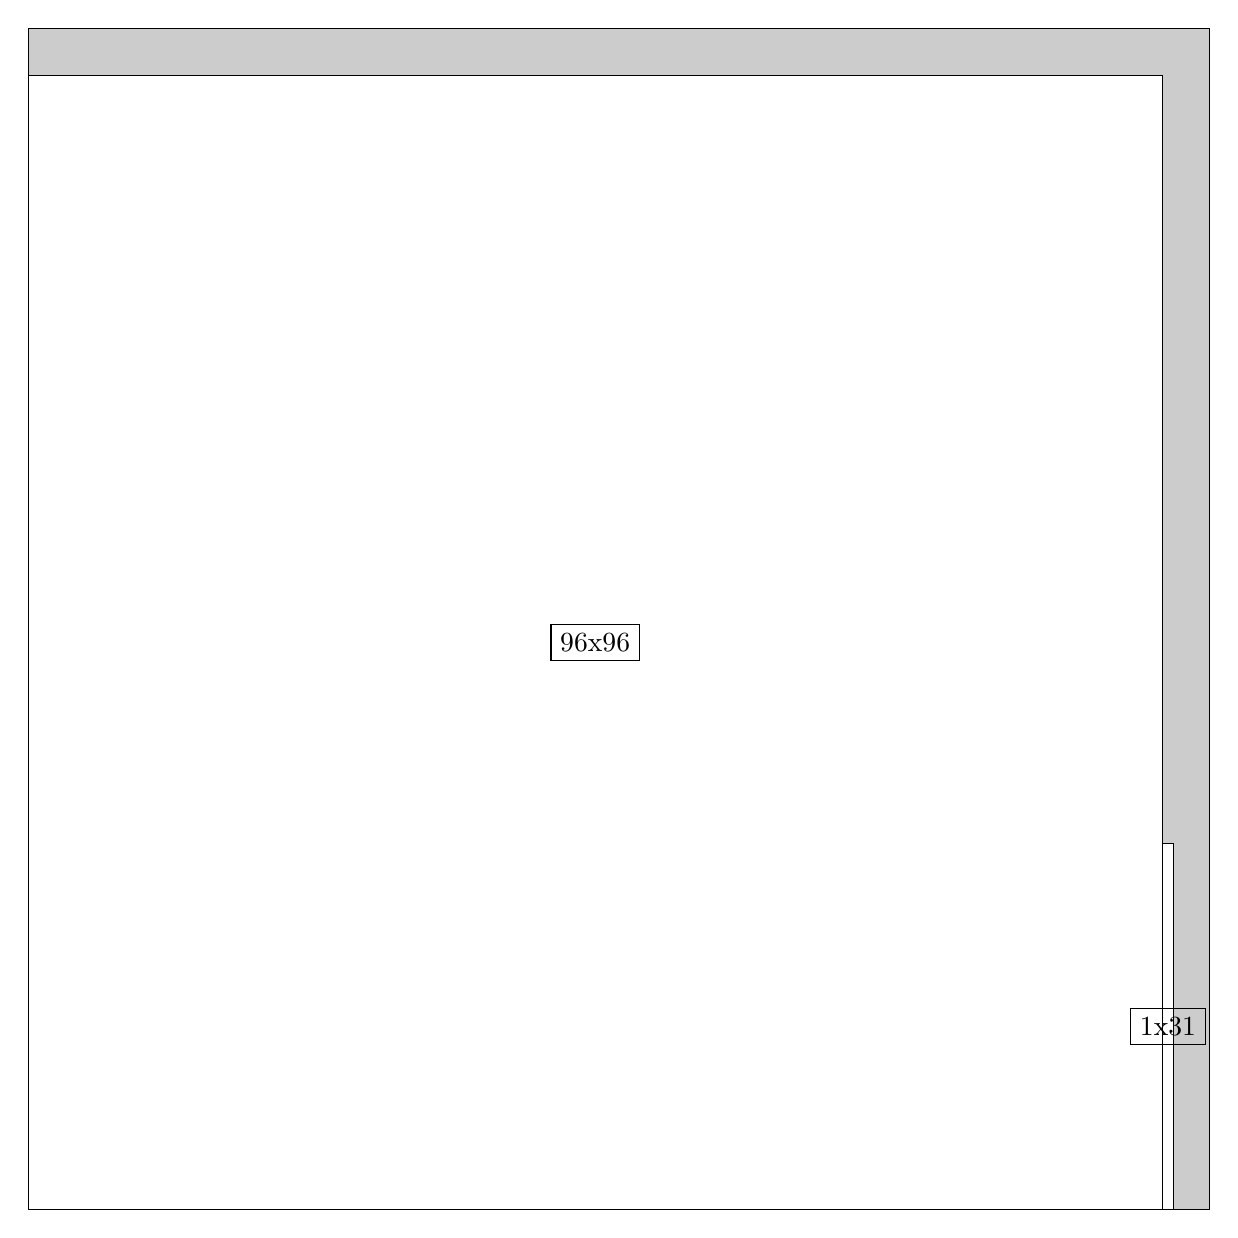
\begin{tikzpicture}[shorten >=1pt,scale=1.0,every node/.style={scale=1.0},->]
\tikzstyle{vertex}=[circle,fill=black!25,minimum size=14pt,inner sep=0pt]
\filldraw[fill=gray!40!white, draw=black] (0,0) rectangle (15.0,15.0);
\foreach \name/\x/\y/\w/\h in {96x96/0.0/0.0/14.399999999999999/14.399999999999999,1x31/14.399999999999999/0.0/0.15/4.6499999999999995}
\filldraw[fill=white!40!white, draw=black] (\x,\y) rectangle node[draw] (\name) {\name} ++(\w,\h);
\end{tikzpicture}


w =96 , h =96 , x =0 , y =0 , v =9216
\par
w =1 , h =31 , x =96 , y =0 , v =31
\par
\newpage


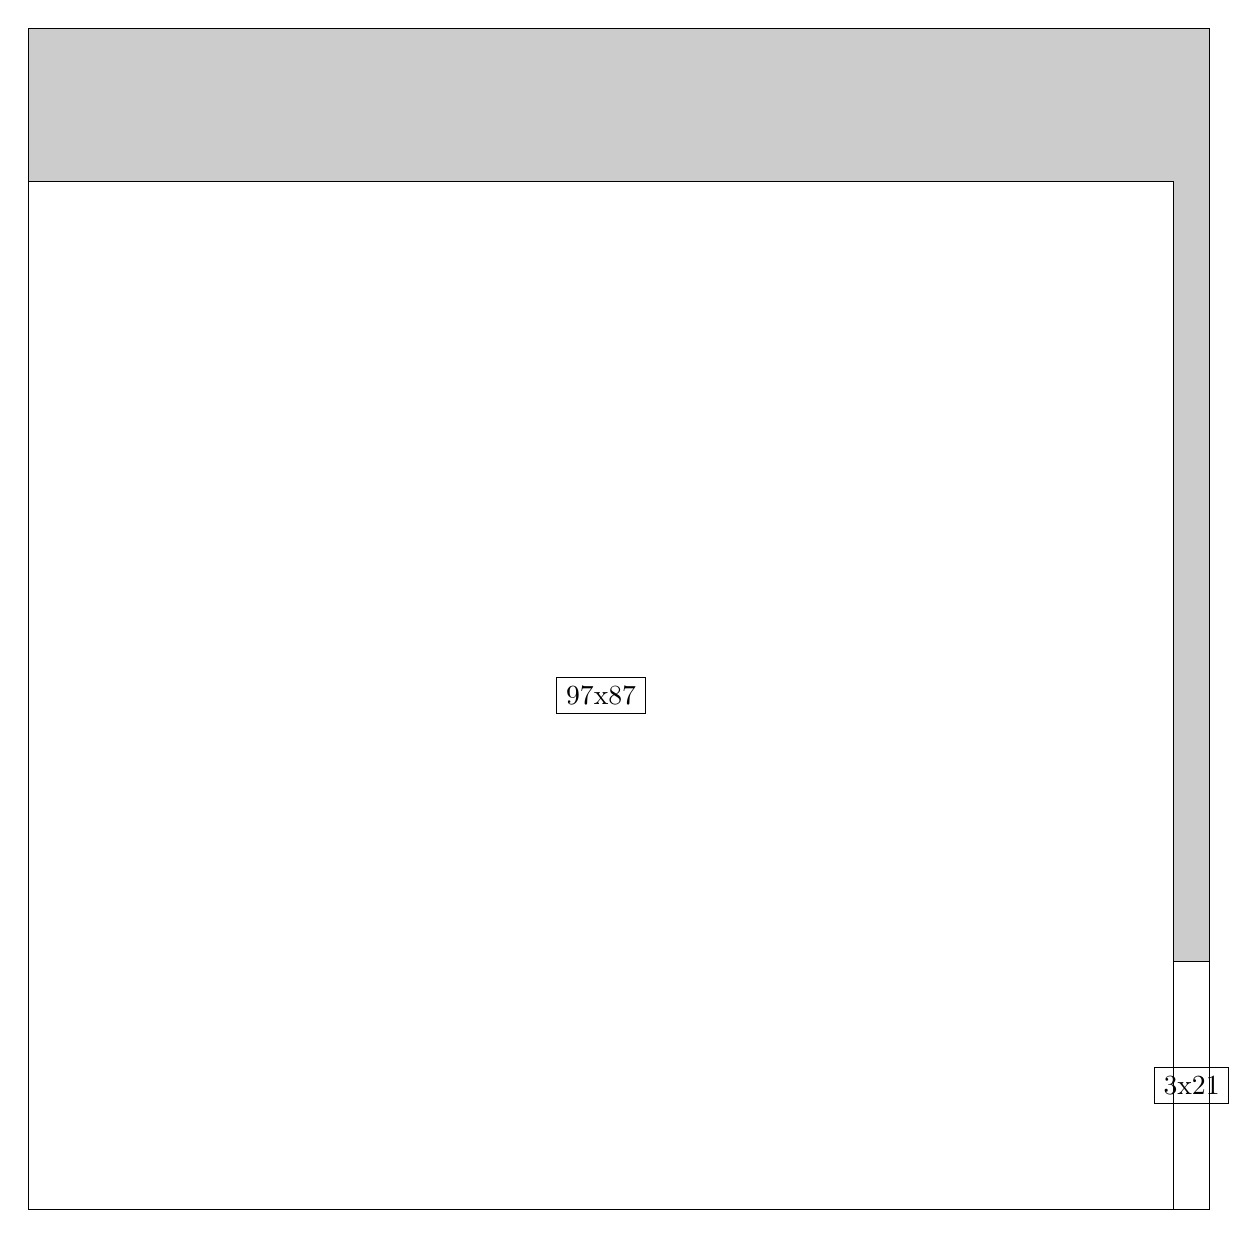
\begin{tikzpicture}[shorten >=1pt,scale=1.0,every node/.style={scale=1.0},->]
\tikzstyle{vertex}=[circle,fill=black!25,minimum size=14pt,inner sep=0pt]
\filldraw[fill=gray!40!white, draw=black] (0,0) rectangle (15.0,15.0);
\foreach \name/\x/\y/\w/\h in {97x87/0.0/0.0/14.549999999999999/13.049999999999999,3x21/14.549999999999999/0.0/0.44999999999999996/3.15}
\filldraw[fill=white!40!white, draw=black] (\x,\y) rectangle node[draw] (\name) {\name} ++(\w,\h);
\end{tikzpicture}


w =97 , h =87 , x =0 , y =0 , v =8439
\par
w =3 , h =21 , x =97 , y =0 , v =63
\par
\newpage


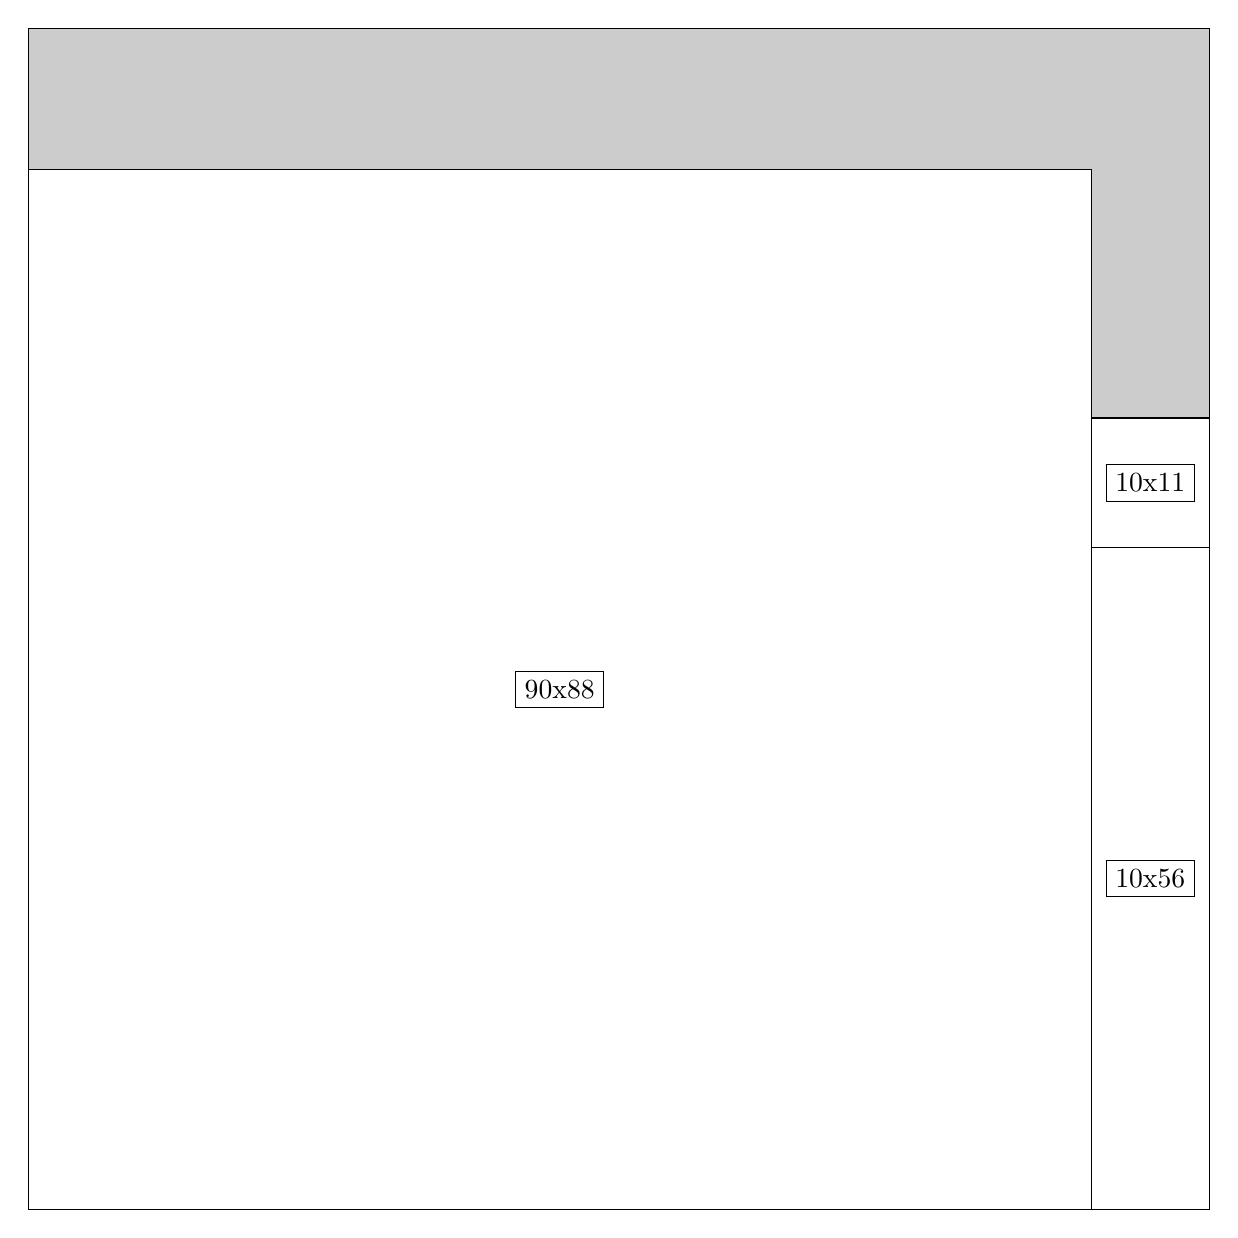
\begin{tikzpicture}[shorten >=1pt,scale=1.0,every node/.style={scale=1.0},->]
\tikzstyle{vertex}=[circle,fill=black!25,minimum size=14pt,inner sep=0pt]
\filldraw[fill=gray!40!white, draw=black] (0,0) rectangle (15.0,15.0);
\foreach \name/\x/\y/\w/\h in {90x88/0.0/0.0/13.5/13.2,10x56/13.5/0.0/1.5/8.4,10x11/13.5/8.4/1.5/1.65}
\filldraw[fill=white!40!white, draw=black] (\x,\y) rectangle node[draw] (\name) {\name} ++(\w,\h);
\end{tikzpicture}


w =90 , h =88 , x =0 , y =0 , v =7920
\par
w =10 , h =56 , x =90 , y =0 , v =560
\par
w =10 , h =11 , x =90 , y =56 , v =110
\par
\newpage


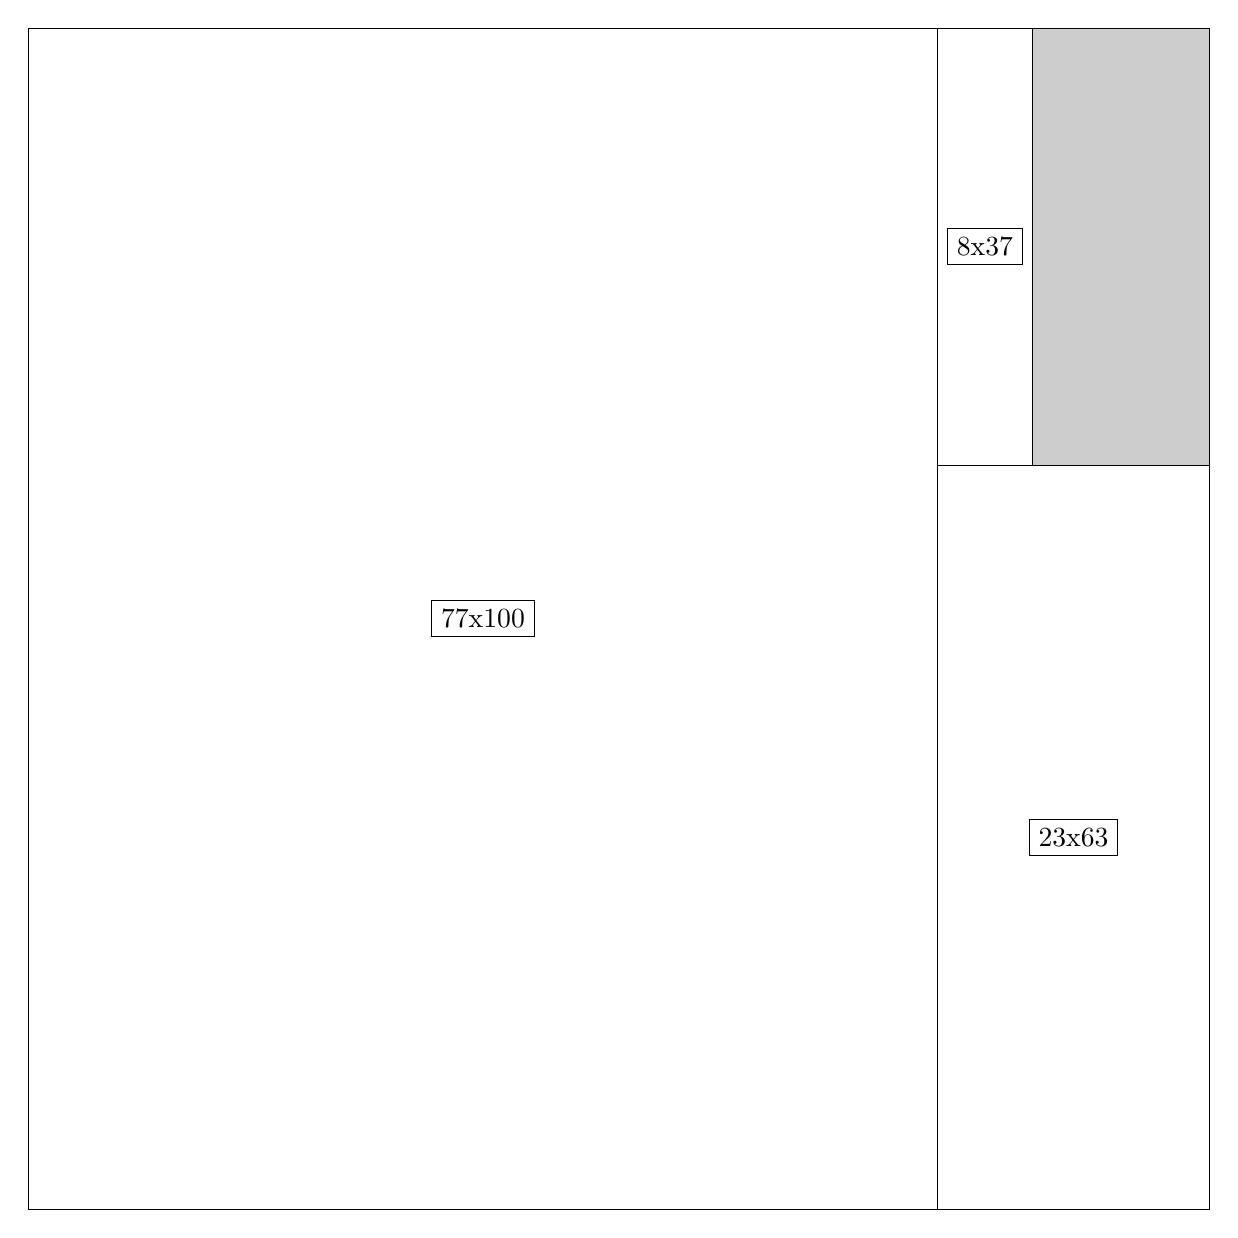
\begin{tikzpicture}[shorten >=1pt,scale=1.0,every node/.style={scale=1.0},->]
\tikzstyle{vertex}=[circle,fill=black!25,minimum size=14pt,inner sep=0pt]
\filldraw[fill=gray!40!white, draw=black] (0,0) rectangle (15.0,15.0);
\foreach \name/\x/\y/\w/\h in {77x100/0.0/0.0/11.549999999999999/15.0,23x63/11.549999999999999/0.0/3.4499999999999997/9.45,8x37/11.549999999999999/9.45/1.2/5.55}
\filldraw[fill=white!40!white, draw=black] (\x,\y) rectangle node[draw] (\name) {\name} ++(\w,\h);
\end{tikzpicture}


w =77 , h =100 , x =0 , y =0 , v =7700
\par
w =23 , h =63 , x =77 , y =0 , v =1449
\par
w =8 , h =37 , x =77 , y =63 , v =296
\par
\newpage


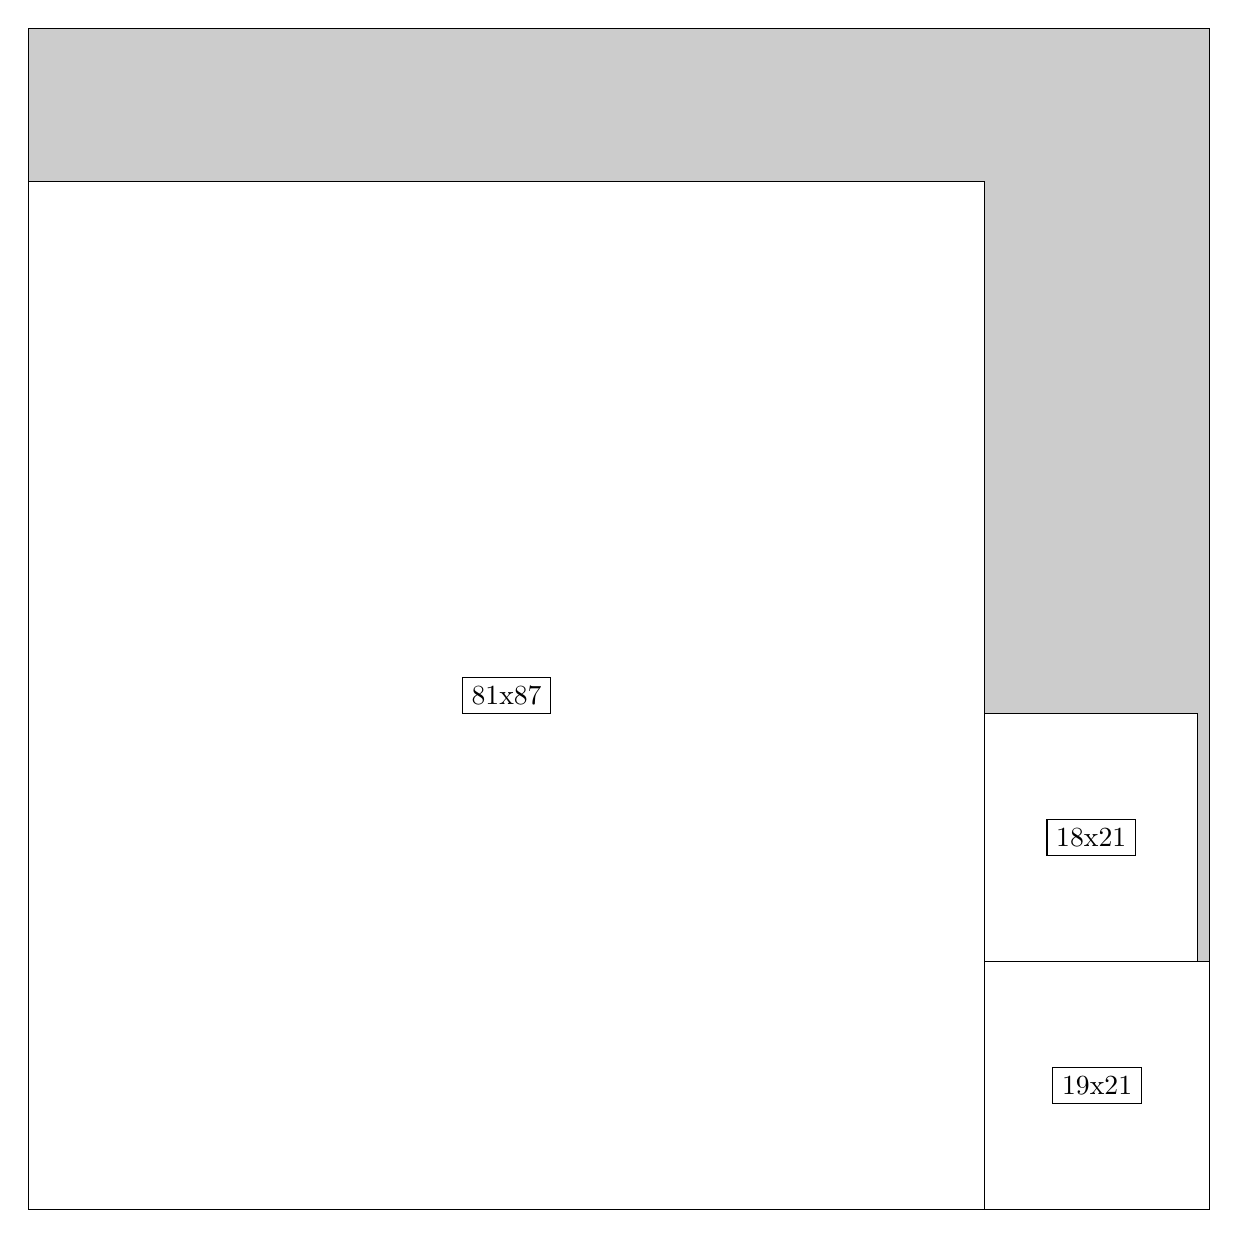
\begin{tikzpicture}[shorten >=1pt,scale=1.0,every node/.style={scale=1.0},->]
\tikzstyle{vertex}=[circle,fill=black!25,minimum size=14pt,inner sep=0pt]
\filldraw[fill=gray!40!white, draw=black] (0,0) rectangle (15.0,15.0);
\foreach \name/\x/\y/\w/\h in {81x87/0.0/0.0/12.15/13.049999999999999,19x21/12.15/0.0/2.85/3.15,18x21/12.15/3.15/2.6999999999999997/3.15}
\filldraw[fill=white!40!white, draw=black] (\x,\y) rectangle node[draw] (\name) {\name} ++(\w,\h);
\end{tikzpicture}


w =81 , h =87 , x =0 , y =0 , v =7047
\par
w =19 , h =21 , x =81 , y =0 , v =399
\par
w =18 , h =21 , x =81 , y =21 , v =378
\par
\newpage


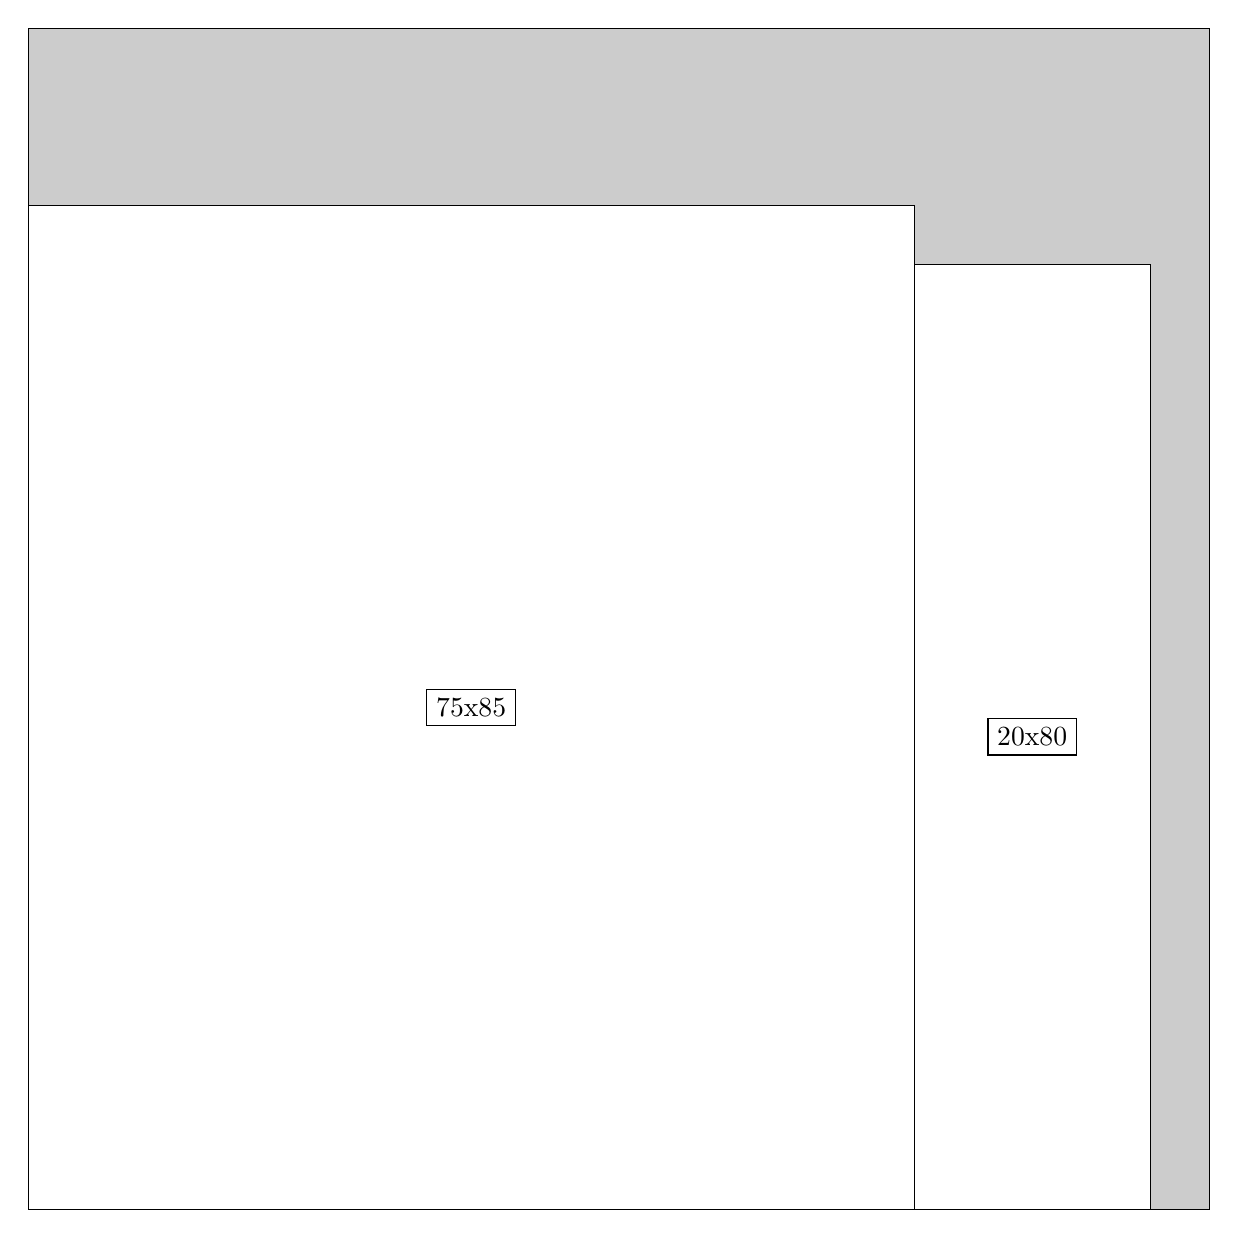
\begin{tikzpicture}[shorten >=1pt,scale=1.0,every node/.style={scale=1.0},->]
\tikzstyle{vertex}=[circle,fill=black!25,minimum size=14pt,inner sep=0pt]
\filldraw[fill=gray!40!white, draw=black] (0,0) rectangle (15.0,15.0);
\foreach \name/\x/\y/\w/\h in {75x85/0.0/0.0/11.25/12.75,20x80/11.25/0.0/3.0/12.0}
\filldraw[fill=white!40!white, draw=black] (\x,\y) rectangle node[draw] (\name) {\name} ++(\w,\h);
\end{tikzpicture}


w =75 , h =85 , x =0 , y =0 , v =6375
\par
w =20 , h =80 , x =75 , y =0 , v =1600
\par
\newpage


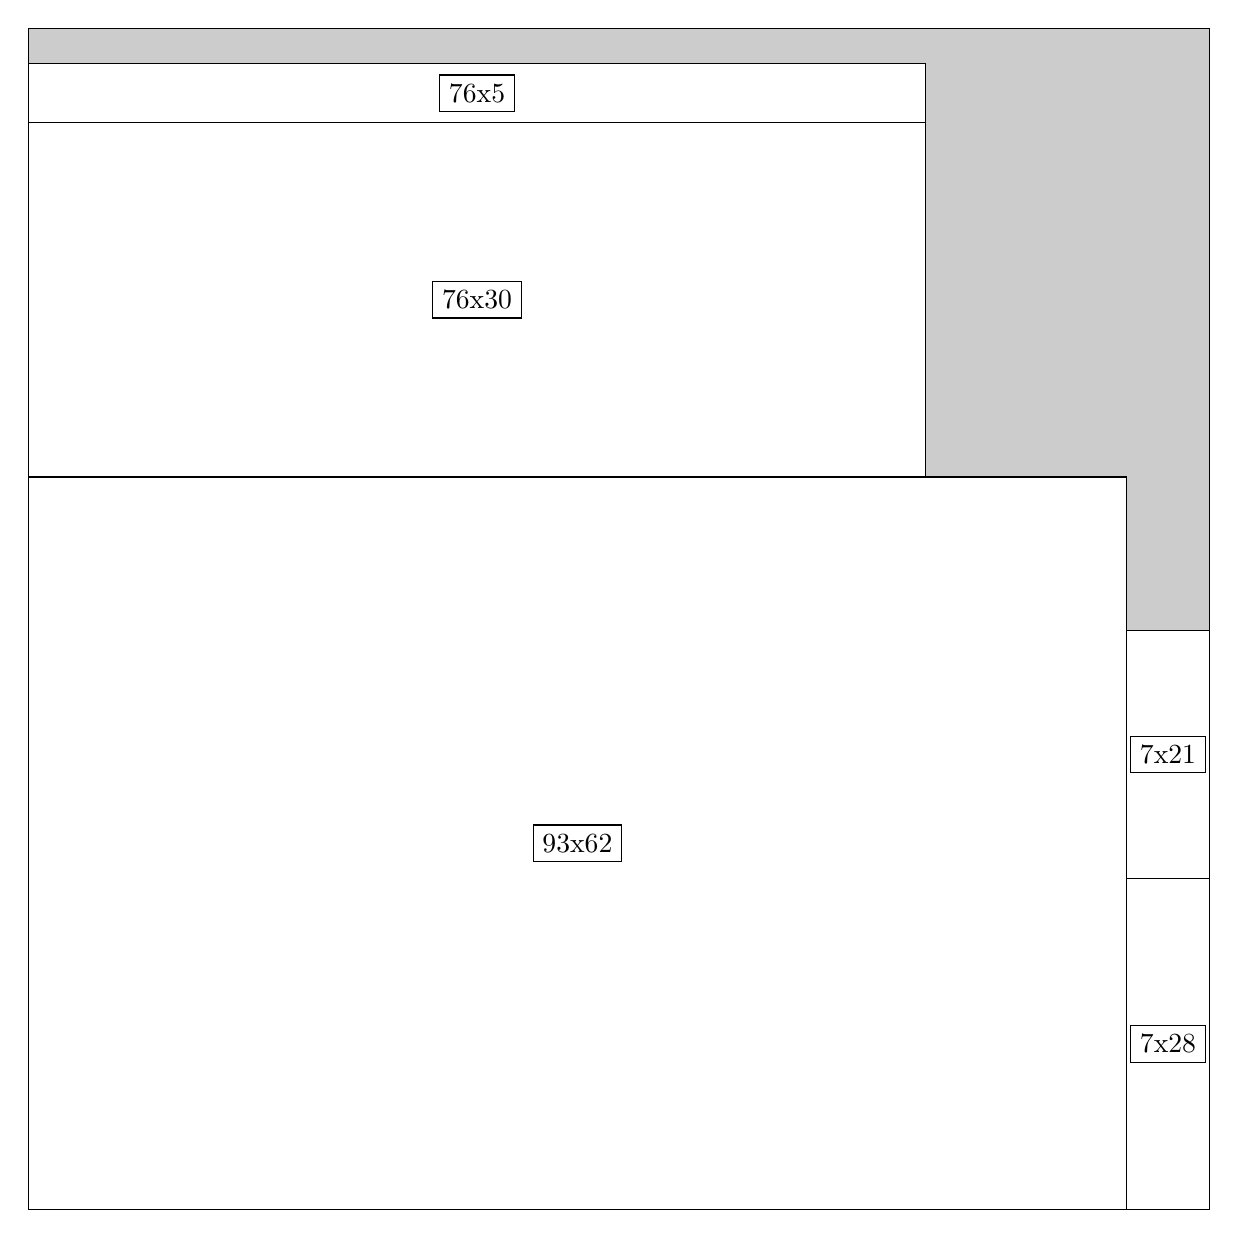
\begin{tikzpicture}[shorten >=1pt,scale=1.0,every node/.style={scale=1.0},->]
\tikzstyle{vertex}=[circle,fill=black!25,minimum size=14pt,inner sep=0pt]
\filldraw[fill=gray!40!white, draw=black] (0,0) rectangle (15.0,15.0);
\foreach \name/\x/\y/\w/\h in {93x62/0.0/0.0/13.95/9.299999999999999,76x30/0.0/9.299999999999999/11.4/4.5,76x5/0.0/13.799999999999999/11.4/0.75,7x28/13.95/0.0/1.05/4.2,7x21/13.95/4.2/1.05/3.15}
\filldraw[fill=white!40!white, draw=black] (\x,\y) rectangle node[draw] (\name) {\name} ++(\w,\h);
\end{tikzpicture}


w =93 , h =62 , x =0 , y =0 , v =5766
\par
w =76 , h =30 , x =0 , y =62 , v =2280
\par
w =76 , h =5 , x =0 , y =92 , v =380
\par
w =7 , h =28 , x =93 , y =0 , v =196
\par
w =7 , h =21 , x =93 , y =28 , v =147
\par
\newpage


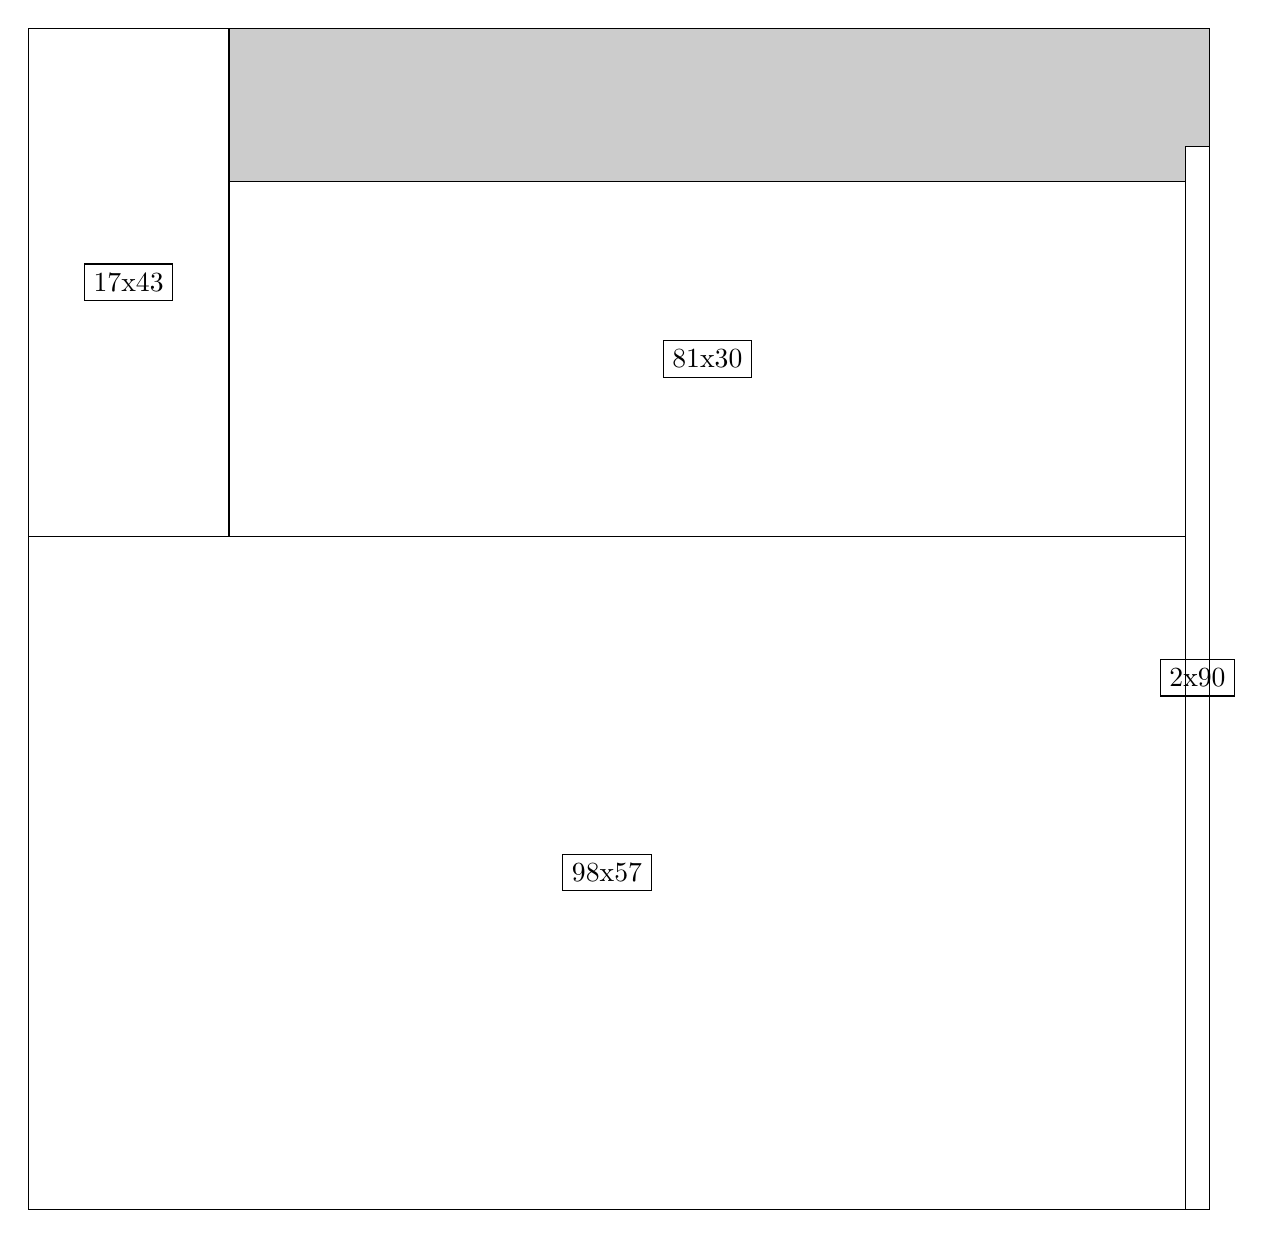
\begin{tikzpicture}[shorten >=1pt,scale=1.0,every node/.style={scale=1.0},->]
\tikzstyle{vertex}=[circle,fill=black!25,minimum size=14pt,inner sep=0pt]
\filldraw[fill=gray!40!white, draw=black] (0,0) rectangle (15.0,15.0);
\foreach \name/\x/\y/\w/\h in {98x57/0.0/0.0/14.7/8.549999999999999,81x30/2.55/8.549999999999999/12.15/4.5,17x43/0.0/8.549999999999999/2.55/6.45,2x90/14.7/0.0/0.3/13.5}
\filldraw[fill=white!40!white, draw=black] (\x,\y) rectangle node[draw] (\name) {\name} ++(\w,\h);
\end{tikzpicture}


w =98 , h =57 , x =0 , y =0 , v =5586
\par
w =81 , h =30 , x =17 , y =57 , v =2430
\par
w =17 , h =43 , x =0 , y =57 , v =731
\par
w =2 , h =90 , x =98 , y =0 , v =180
\par
\newpage


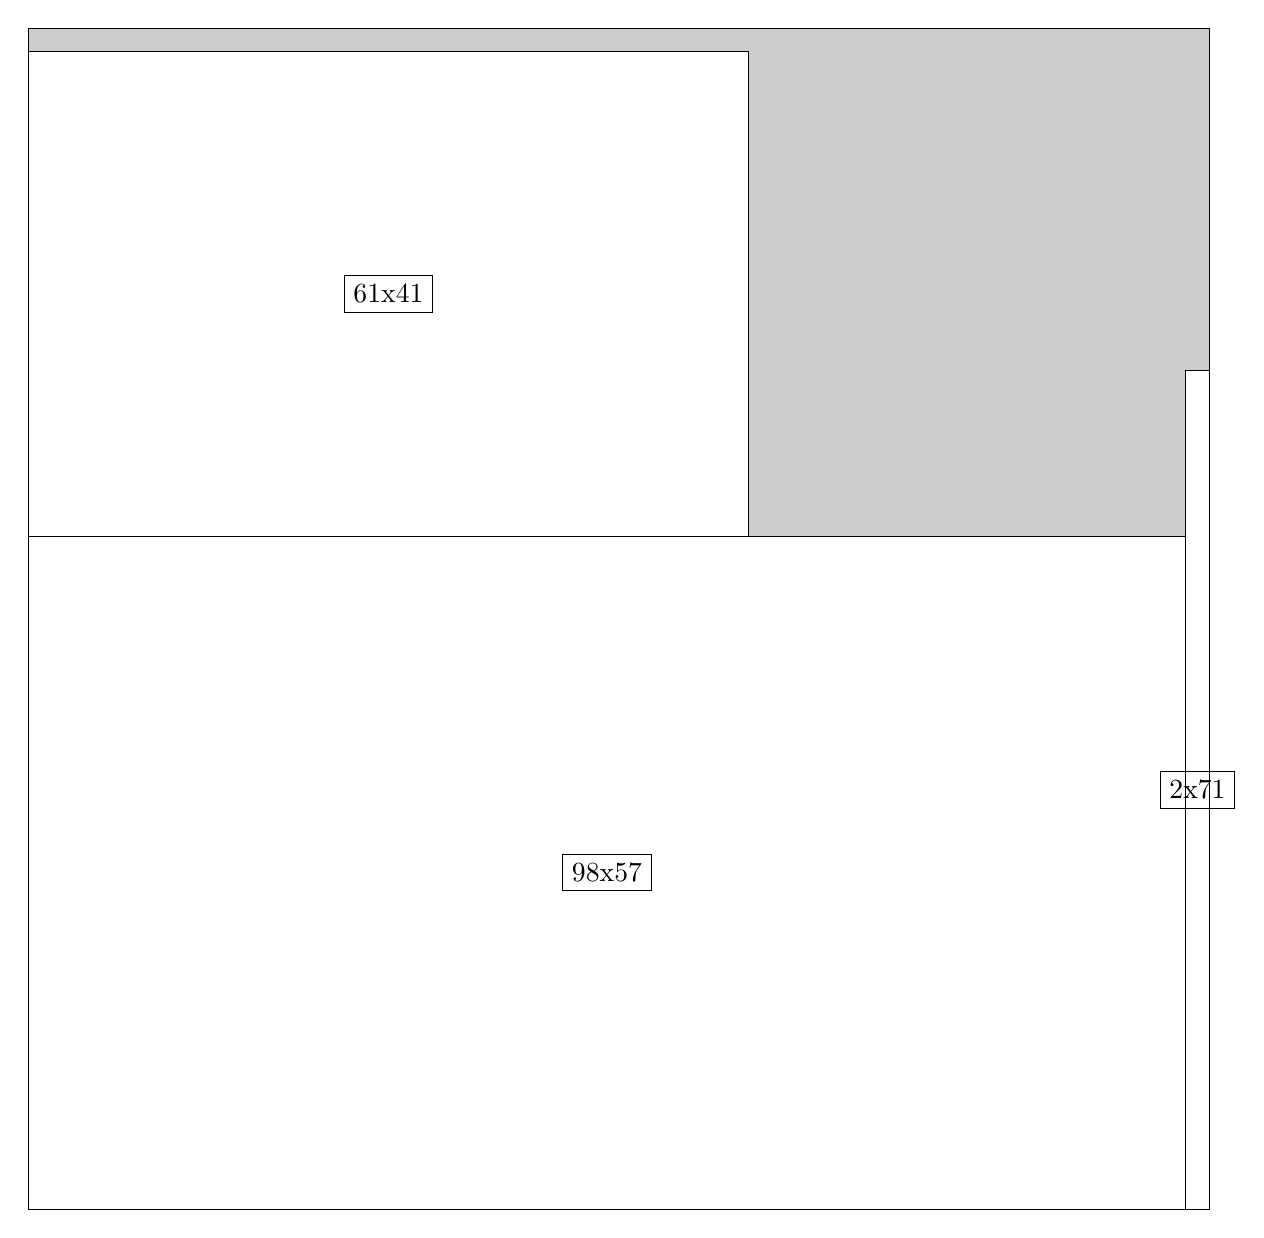
\begin{tikzpicture}[shorten >=1pt,scale=1.0,every node/.style={scale=1.0},->]
\tikzstyle{vertex}=[circle,fill=black!25,minimum size=14pt,inner sep=0pt]
\filldraw[fill=gray!40!white, draw=black] (0,0) rectangle (15.0,15.0);
\foreach \name/\x/\y/\w/\h in {98x57/0.0/0.0/14.7/8.549999999999999,61x41/0.0/8.549999999999999/9.15/6.1499999999999995,2x71/14.7/0.0/0.3/10.65}
\filldraw[fill=white!40!white, draw=black] (\x,\y) rectangle node[draw] (\name) {\name} ++(\w,\h);
\end{tikzpicture}


w =98 , h =57 , x =0 , y =0 , v =5586
\par
w =61 , h =41 , x =0 , y =57 , v =2501
\par
w =2 , h =71 , x =98 , y =0 , v =142
\par
\newpage


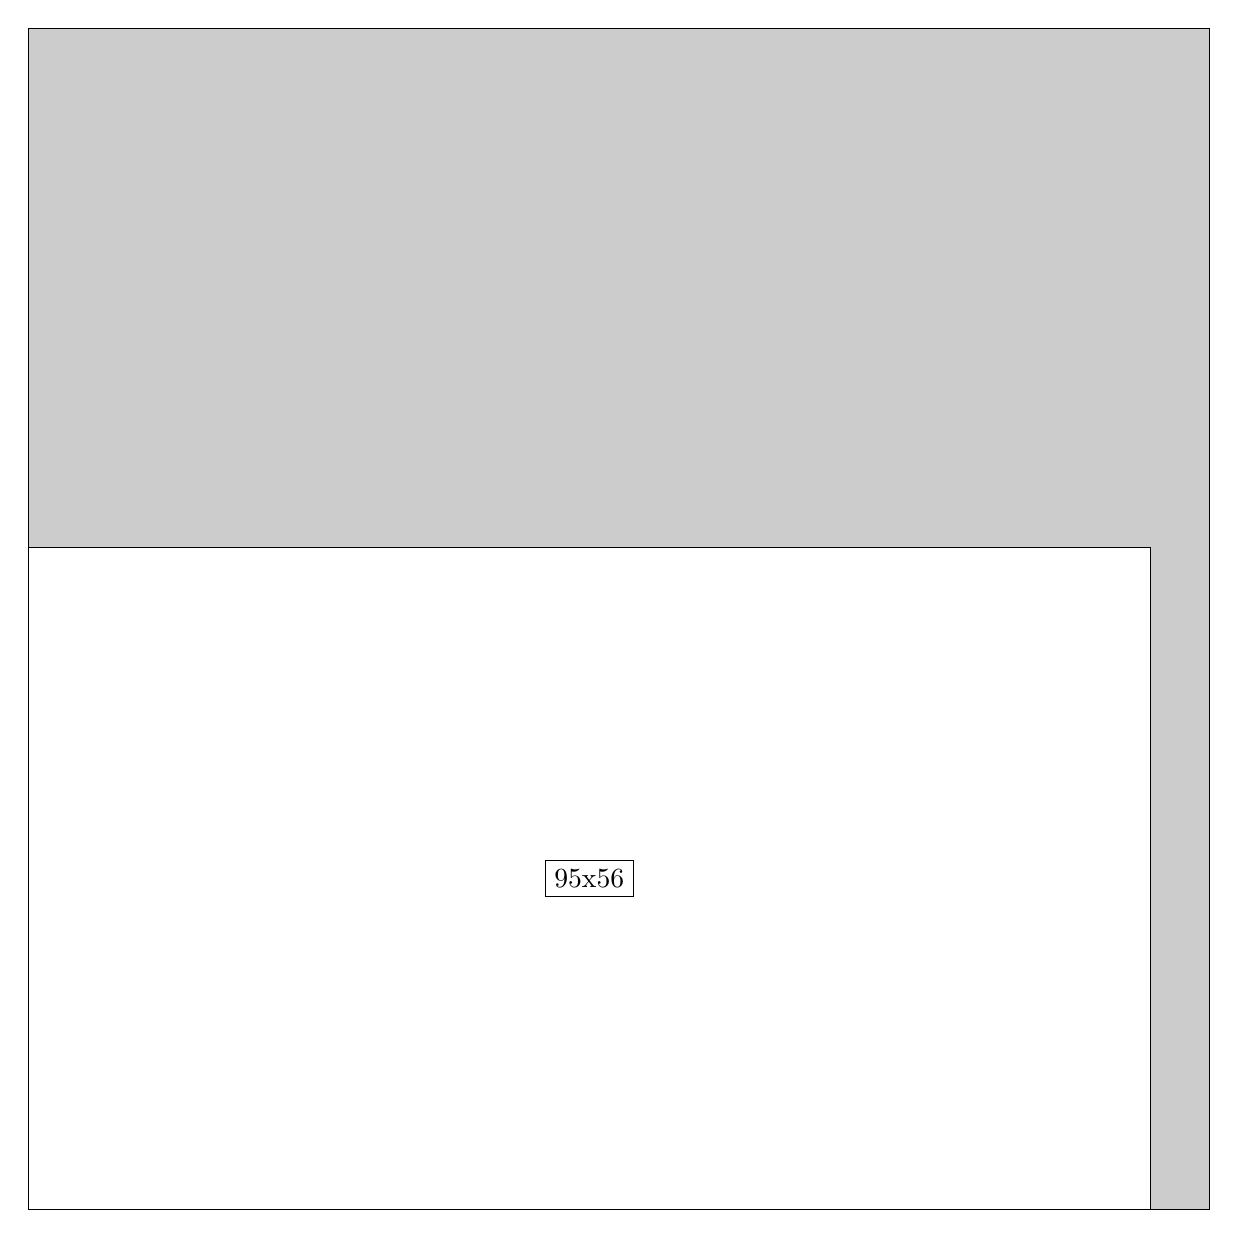
\begin{tikzpicture}[shorten >=1pt,scale=1.0,every node/.style={scale=1.0},->]
\tikzstyle{vertex}=[circle,fill=black!25,minimum size=14pt,inner sep=0pt]
\filldraw[fill=gray!40!white, draw=black] (0,0) rectangle (15.0,15.0);
\foreach \name/\x/\y/\w/\h in {95x56/0.0/0.0/14.25/8.4}
\filldraw[fill=white!40!white, draw=black] (\x,\y) rectangle node[draw] (\name) {\name} ++(\w,\h);
\end{tikzpicture}


w =95 , h =56 , x =0 , y =0 , v =5320
\par
\newpage


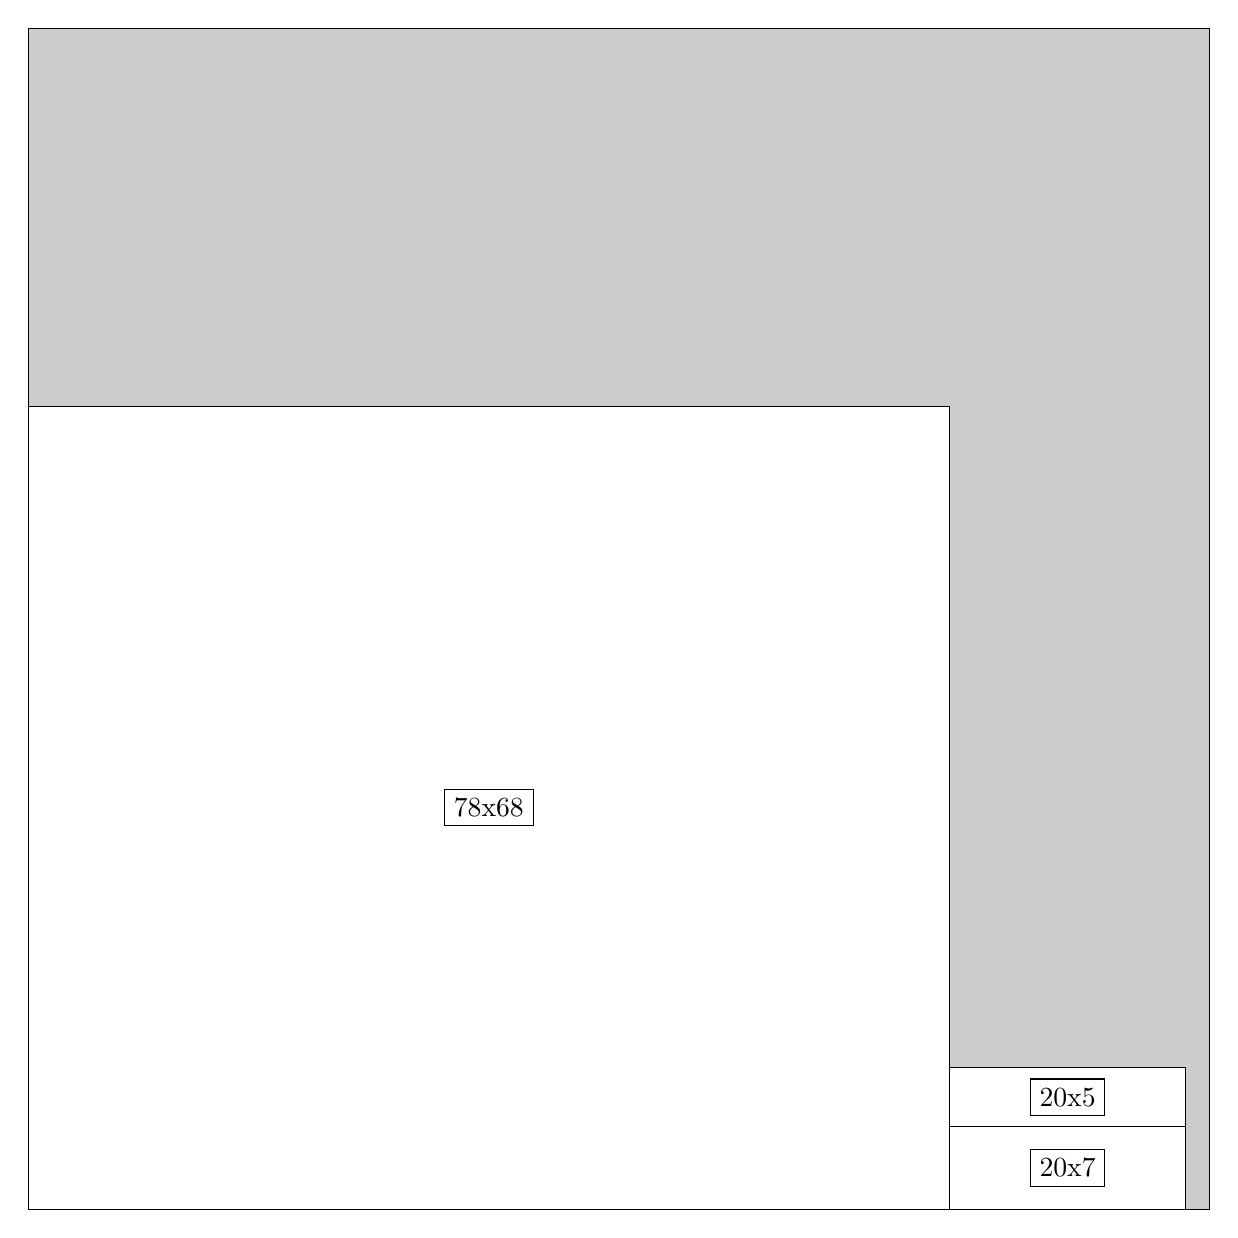
\begin{tikzpicture}[shorten >=1pt,scale=1.0,every node/.style={scale=1.0},->]
\tikzstyle{vertex}=[circle,fill=black!25,minimum size=14pt,inner sep=0pt]
\filldraw[fill=gray!40!white, draw=black] (0,0) rectangle (15.0,15.0);
\foreach \name/\x/\y/\w/\h in {78x68/0.0/0.0/11.7/10.2,20x7/11.7/0.0/3.0/1.05,20x5/11.7/1.05/3.0/0.75}
\filldraw[fill=white!40!white, draw=black] (\x,\y) rectangle node[draw] (\name) {\name} ++(\w,\h);
\end{tikzpicture}


w =78 , h =68 , x =0 , y =0 , v =5304
\par
w =20 , h =7 , x =78 , y =0 , v =140
\par
w =20 , h =5 , x =78 , y =7 , v =100
\par
\newpage


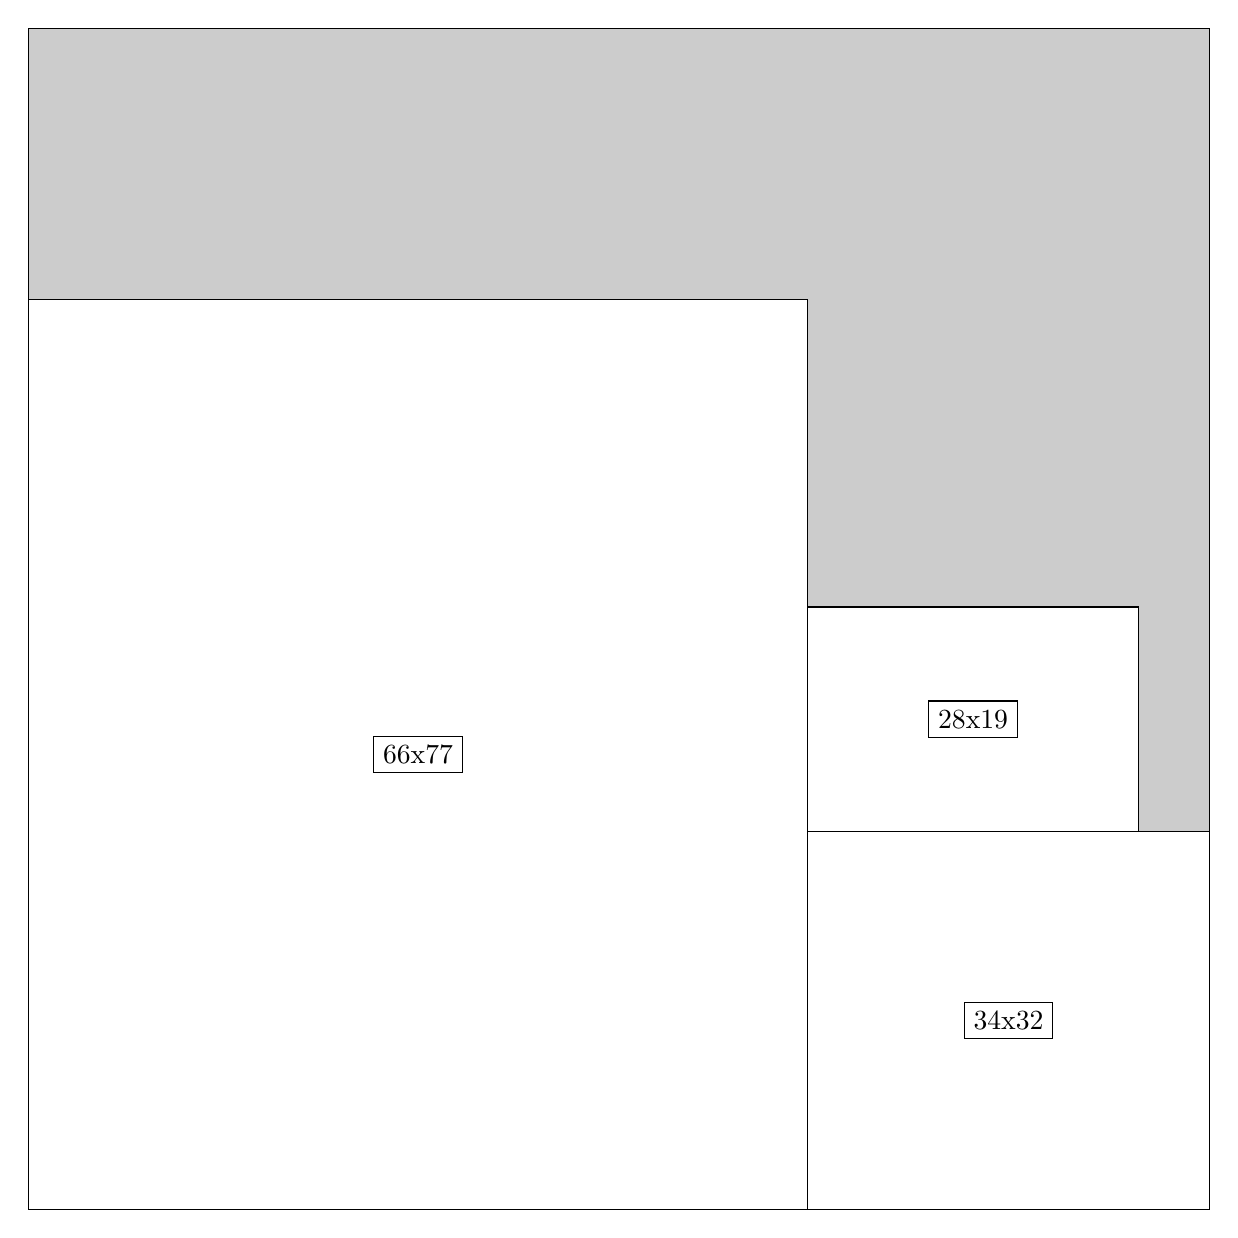
\begin{tikzpicture}[shorten >=1pt,scale=1.0,every node/.style={scale=1.0},->]
\tikzstyle{vertex}=[circle,fill=black!25,minimum size=14pt,inner sep=0pt]
\filldraw[fill=gray!40!white, draw=black] (0,0) rectangle (15.0,15.0);
\foreach \name/\x/\y/\w/\h in {66x77/0.0/0.0/9.9/11.549999999999999,34x32/9.9/0.0/5.1/4.8,28x19/9.9/4.8/4.2/2.85}
\filldraw[fill=white!40!white, draw=black] (\x,\y) rectangle node[draw] (\name) {\name} ++(\w,\h);
\end{tikzpicture}


w =66 , h =77 , x =0 , y =0 , v =5082
\par
w =34 , h =32 , x =66 , y =0 , v =1088
\par
w =28 , h =19 , x =66 , y =32 , v =532
\par
\newpage


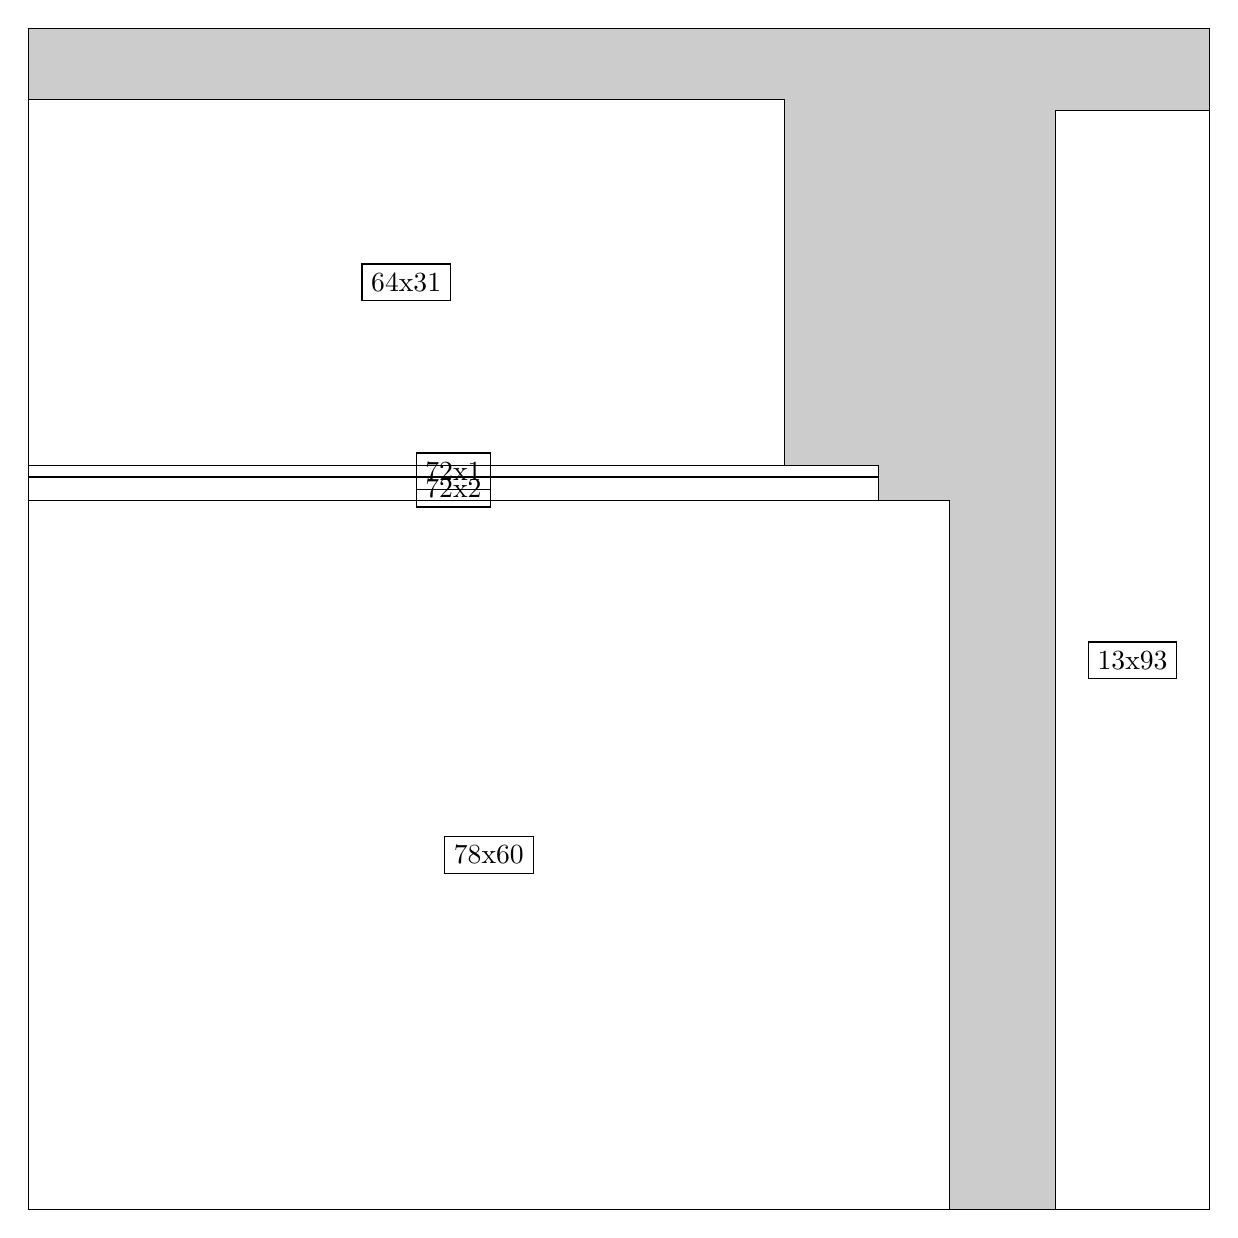
\begin{tikzpicture}[shorten >=1pt,scale=1.0,every node/.style={scale=1.0},->]
\tikzstyle{vertex}=[circle,fill=black!25,minimum size=14pt,inner sep=0pt]
\filldraw[fill=gray!40!white, draw=black] (0,0) rectangle (15.0,15.0);
\foreach \name/\x/\y/\w/\h in {78x60/0.0/0.0/11.7/9.0,64x31/0.0/9.45/9.6/4.6499999999999995,13x93/13.049999999999999/0.0/1.95/13.95,72x2/0.0/9.0/10.799999999999999/0.3,72x1/0.0/9.299999999999999/10.799999999999999/0.15}
\filldraw[fill=white!40!white, draw=black] (\x,\y) rectangle node[draw] (\name) {\name} ++(\w,\h);
\end{tikzpicture}


w =78 , h =60 , x =0 , y =0 , v =4680
\par
w =64 , h =31 , x =0 , y =63 , v =1984
\par
w =13 , h =93 , x =87 , y =0 , v =1209
\par
w =72 , h =2 , x =0 , y =60 , v =144
\par
w =72 , h =1 , x =0 , y =62 , v =72
\par
\newpage


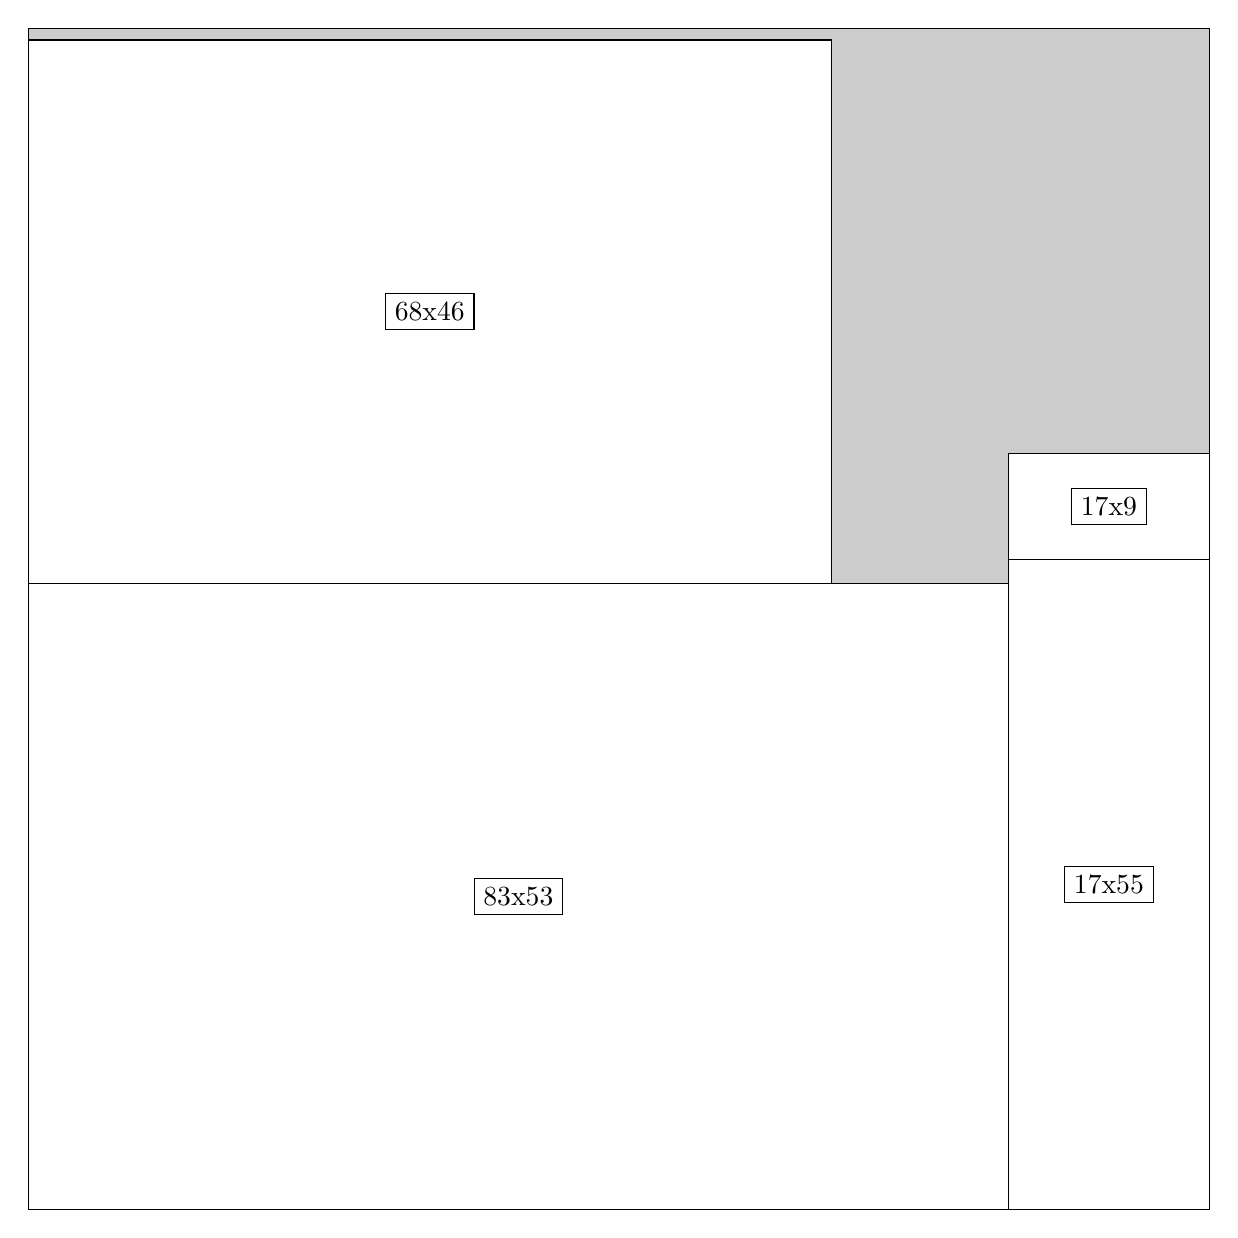
\begin{tikzpicture}[shorten >=1pt,scale=1.0,every node/.style={scale=1.0},->]
\tikzstyle{vertex}=[circle,fill=black!25,minimum size=14pt,inner sep=0pt]
\filldraw[fill=gray!40!white, draw=black] (0,0) rectangle (15.0,15.0);
\foreach \name/\x/\y/\w/\h in {83x53/0.0/0.0/12.45/7.949999999999999,68x46/0.0/7.949999999999999/10.2/6.8999999999999995,17x55/12.45/0.0/2.55/8.25,17x9/12.45/8.25/2.55/1.3499999999999999}
\filldraw[fill=white!40!white, draw=black] (\x,\y) rectangle node[draw] (\name) {\name} ++(\w,\h);
\end{tikzpicture}


w =83 , h =53 , x =0 , y =0 , v =4399
\par
w =68 , h =46 , x =0 , y =53 , v =3128
\par
w =17 , h =55 , x =83 , y =0 , v =935
\par
w =17 , h =9 , x =83 , y =55 , v =153
\par
\newpage


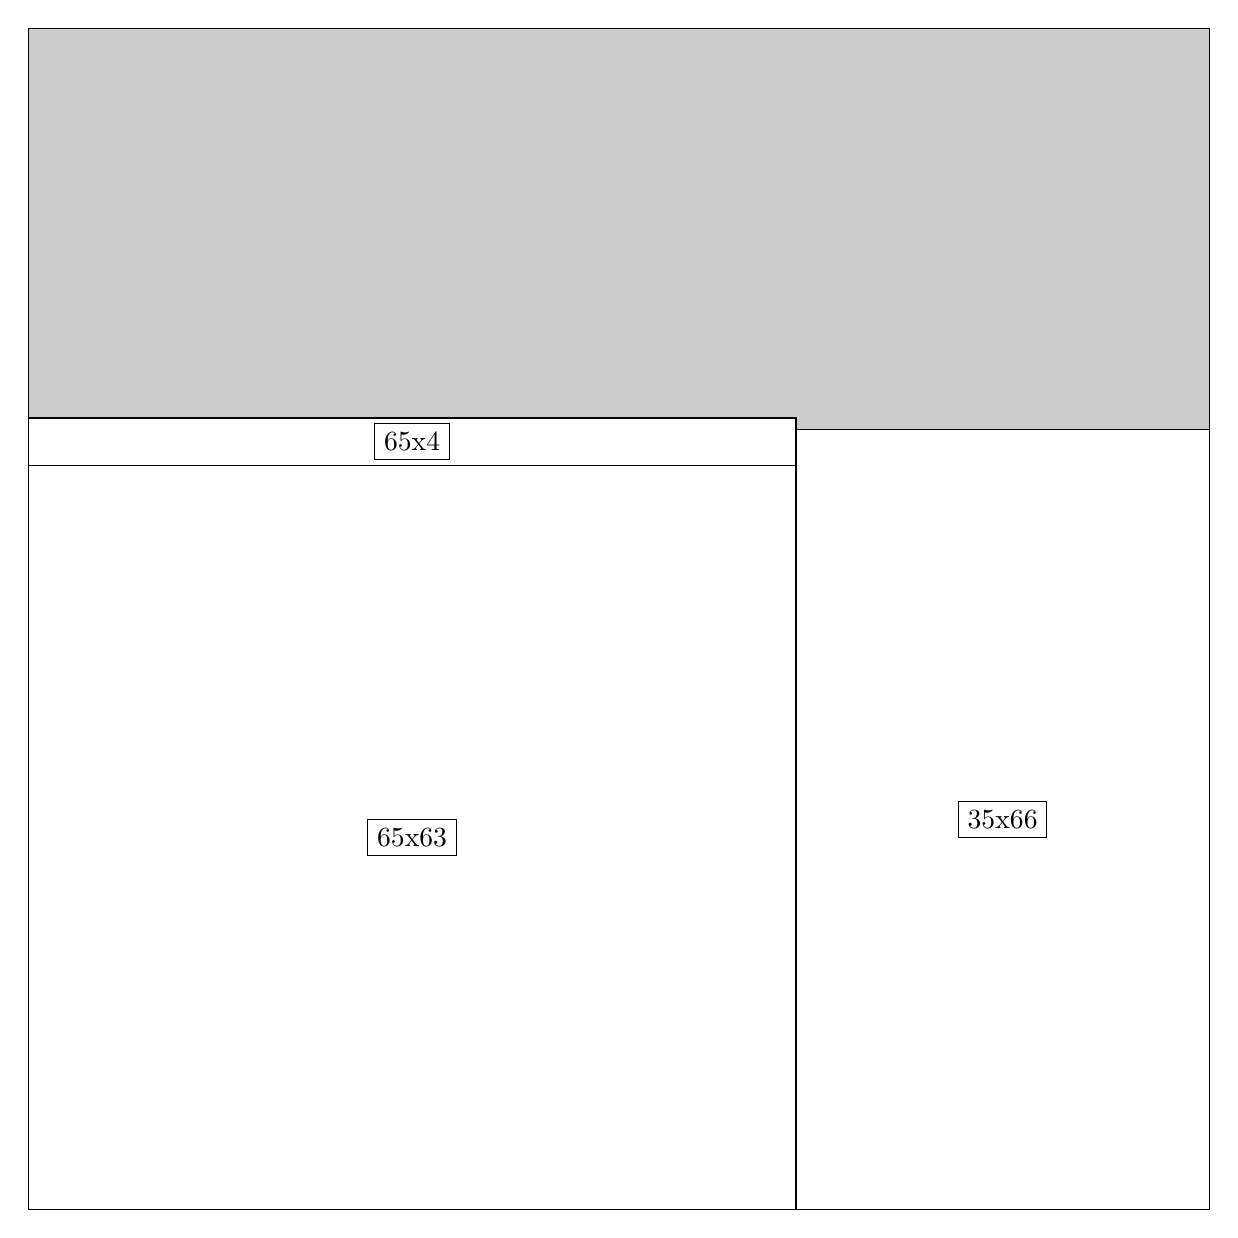
\begin{tikzpicture}[shorten >=1pt,scale=1.0,every node/.style={scale=1.0},->]
\tikzstyle{vertex}=[circle,fill=black!25,minimum size=14pt,inner sep=0pt]
\filldraw[fill=gray!40!white, draw=black] (0,0) rectangle (15.0,15.0);
\foreach \name/\x/\y/\w/\h in {65x63/0.0/0.0/9.75/9.45,35x66/9.75/0.0/5.25/9.9,65x4/0.0/9.45/9.75/0.6}
\filldraw[fill=white!40!white, draw=black] (\x,\y) rectangle node[draw] (\name) {\name} ++(\w,\h);
\end{tikzpicture}


w =65 , h =63 , x =0 , y =0 , v =4095
\par
w =35 , h =66 , x =65 , y =0 , v =2310
\par
w =65 , h =4 , x =0 , y =63 , v =260
\par
\newpage


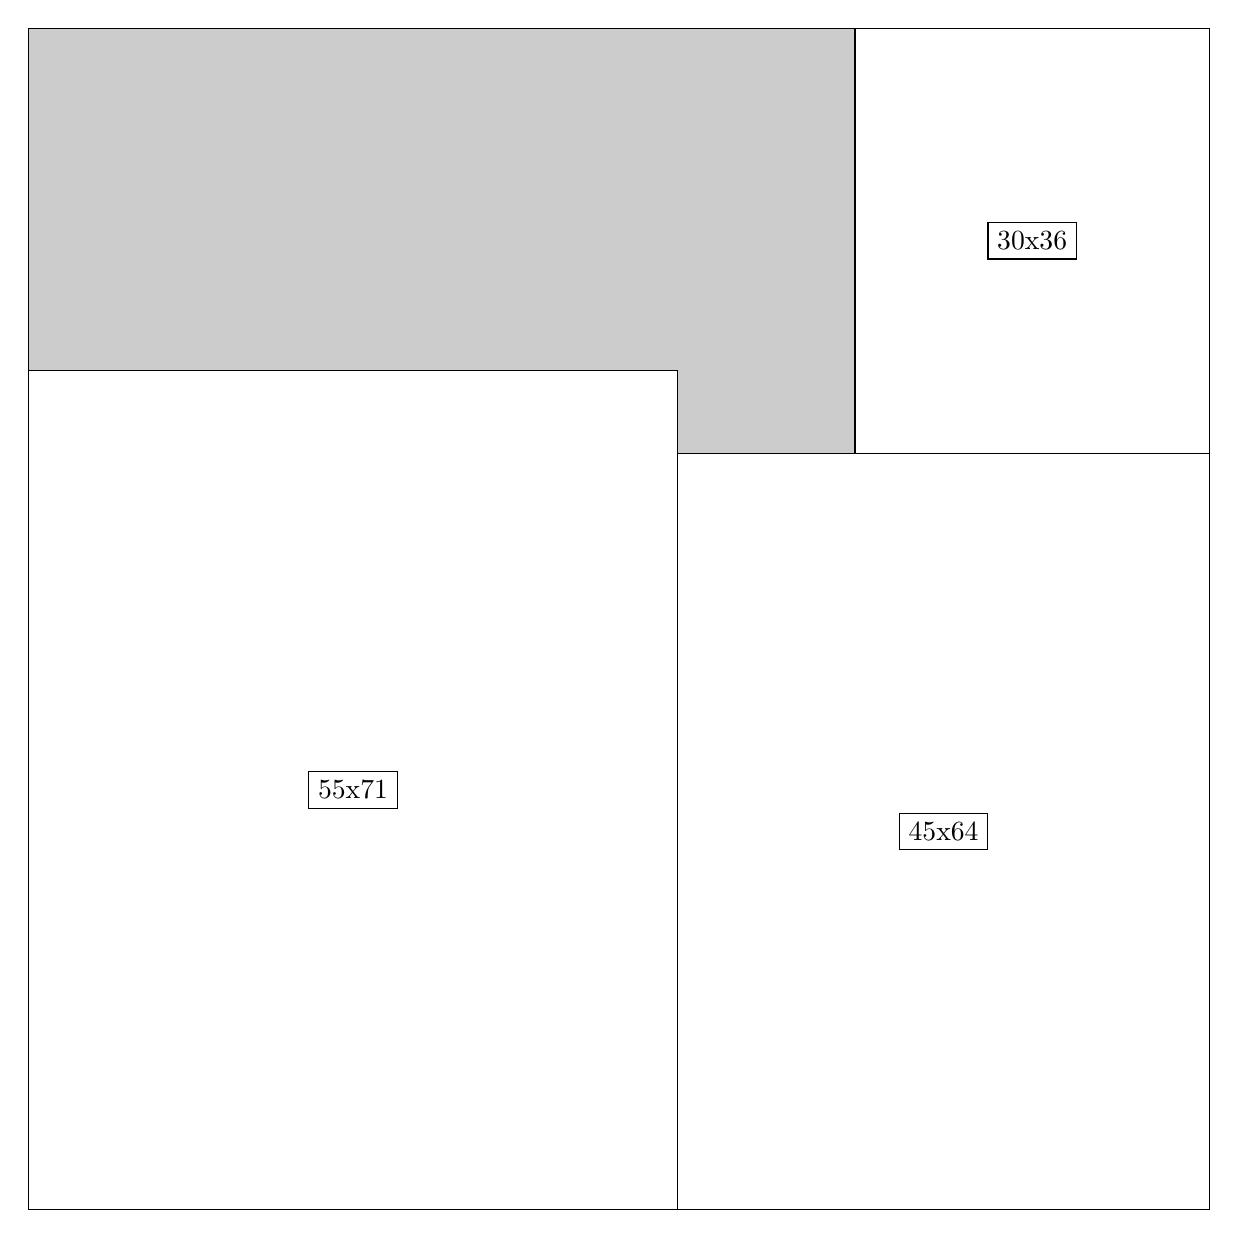
\begin{tikzpicture}[shorten >=1pt,scale=1.0,every node/.style={scale=1.0},->]
\tikzstyle{vertex}=[circle,fill=black!25,minimum size=14pt,inner sep=0pt]
\filldraw[fill=gray!40!white, draw=black] (0,0) rectangle (15.0,15.0);
\foreach \name/\x/\y/\w/\h in {55x71/0.0/0.0/8.25/10.65,45x64/8.25/0.0/6.75/9.6,30x36/10.5/9.6/4.5/5.3999999999999995}
\filldraw[fill=white!40!white, draw=black] (\x,\y) rectangle node[draw] (\name) {\name} ++(\w,\h);
\end{tikzpicture}


w =55 , h =71 , x =0 , y =0 , v =3905
\par
w =45 , h =64 , x =55 , y =0 , v =2880
\par
w =30 , h =36 , x =70 , y =64 , v =1080
\par
\newpage


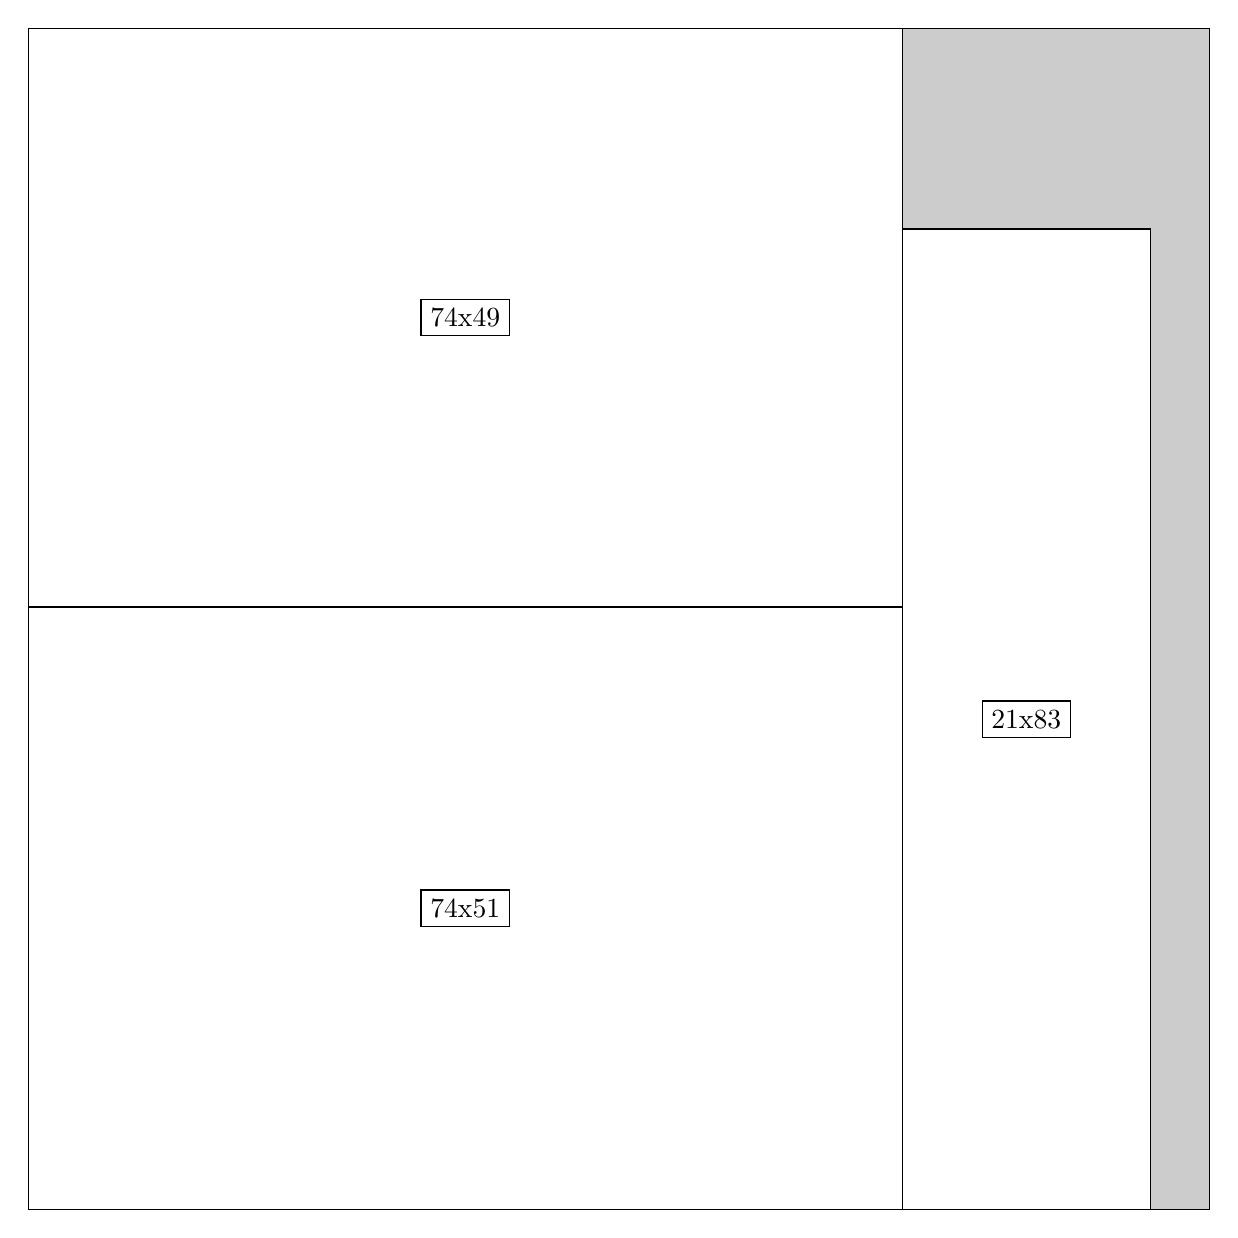
\begin{tikzpicture}[shorten >=1pt,scale=1.0,every node/.style={scale=1.0},->]
\tikzstyle{vertex}=[circle,fill=black!25,minimum size=14pt,inner sep=0pt]
\filldraw[fill=gray!40!white, draw=black] (0,0) rectangle (15.0,15.0);
\foreach \name/\x/\y/\w/\h in {74x51/0.0/0.0/11.1/7.6499999999999995,74x49/0.0/7.6499999999999995/11.1/7.35,21x83/11.1/0.0/3.15/12.45}
\filldraw[fill=white!40!white, draw=black] (\x,\y) rectangle node[draw] (\name) {\name} ++(\w,\h);
\end{tikzpicture}


w =74 , h =51 , x =0 , y =0 , v =3774
\par
w =74 , h =49 , x =0 , y =51 , v =3626
\par
w =21 , h =83 , x =74 , y =0 , v =1743
\par
\newpage


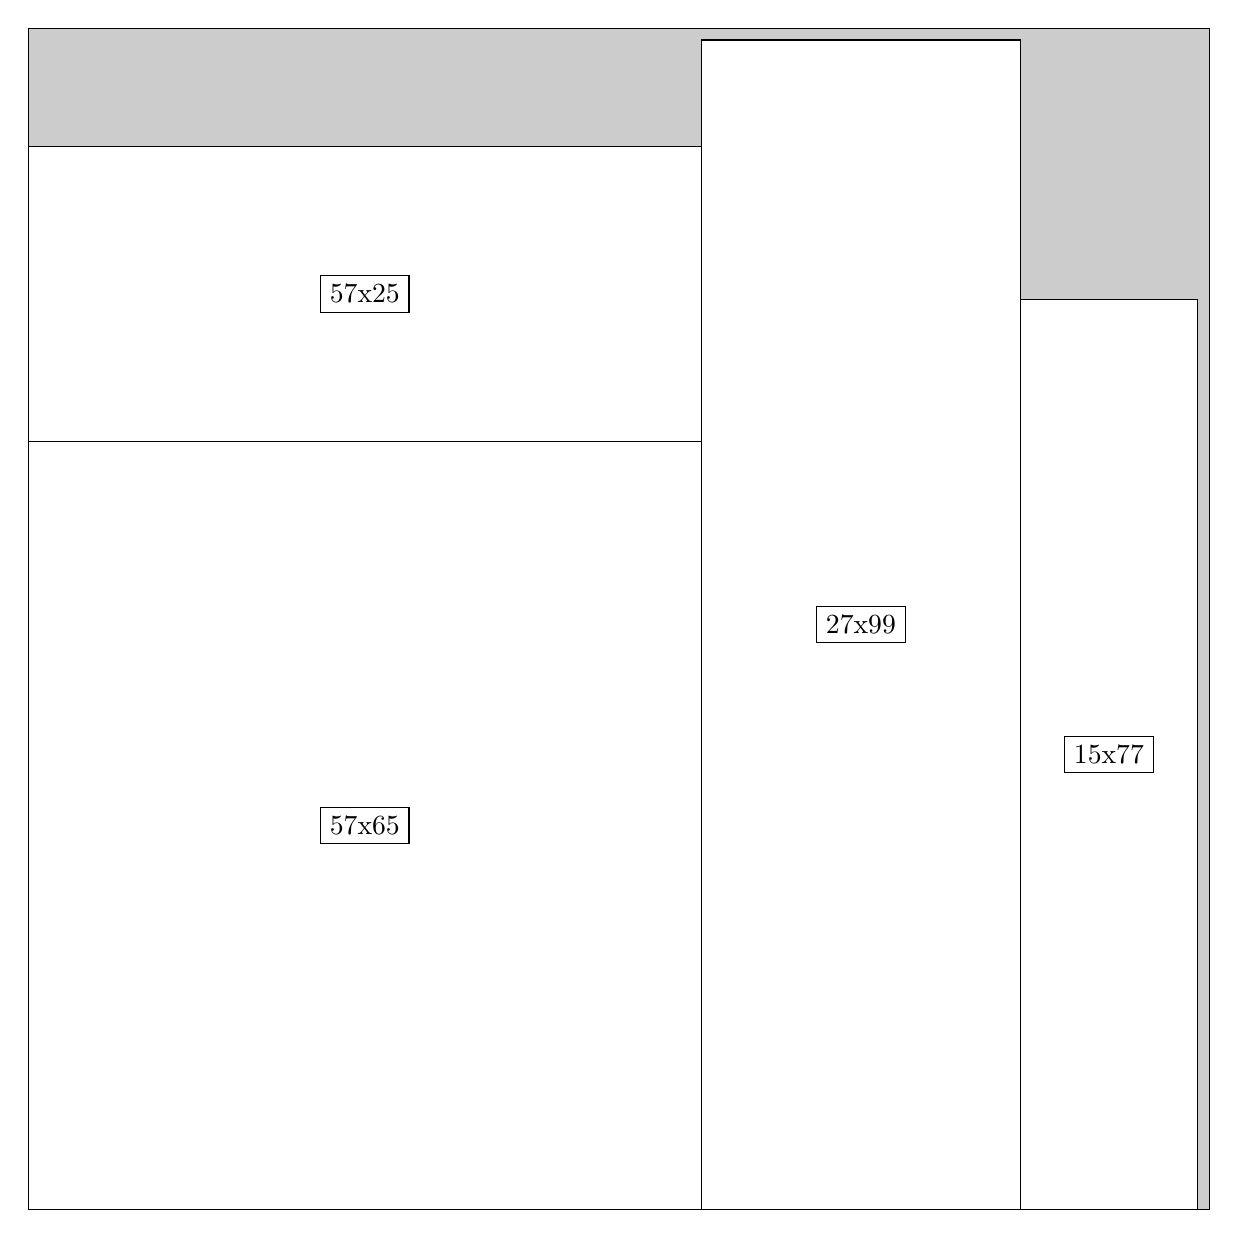
\begin{tikzpicture}[shorten >=1pt,scale=1.0,every node/.style={scale=1.0},->]
\tikzstyle{vertex}=[circle,fill=black!25,minimum size=14pt,inner sep=0pt]
\filldraw[fill=gray!40!white, draw=black] (0,0) rectangle (15.0,15.0);
\foreach \name/\x/\y/\w/\h in {57x65/0.0/0.0/8.549999999999999/9.75,27x99/8.549999999999999/0.0/4.05/14.85,57x25/0.0/9.75/8.549999999999999/3.75,15x77/12.6/0.0/2.25/11.549999999999999}
\filldraw[fill=white!40!white, draw=black] (\x,\y) rectangle node[draw] (\name) {\name} ++(\w,\h);
\end{tikzpicture}


w =57 , h =65 , x =0 , y =0 , v =3705
\par
w =27 , h =99 , x =57 , y =0 , v =2673
\par
w =57 , h =25 , x =0 , y =65 , v =1425
\par
w =15 , h =77 , x =84 , y =0 , v =1155
\par
\newpage


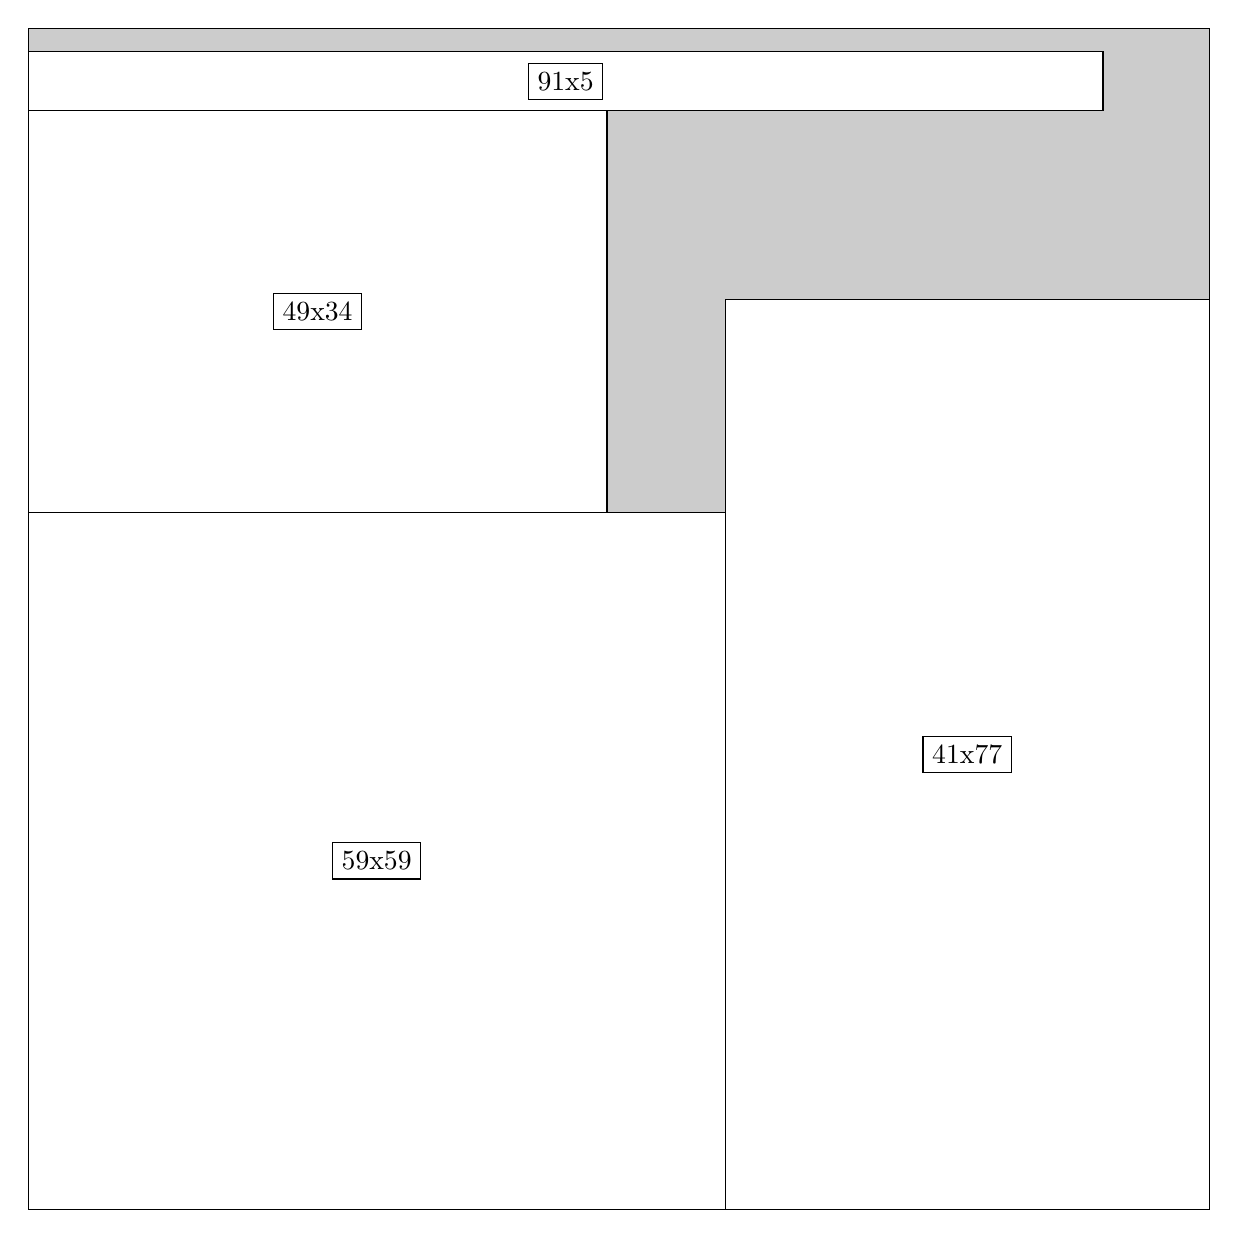
\begin{tikzpicture}[shorten >=1pt,scale=1.0,every node/.style={scale=1.0},->]
\tikzstyle{vertex}=[circle,fill=black!25,minimum size=14pt,inner sep=0pt]
\filldraw[fill=gray!40!white, draw=black] (0,0) rectangle (15.0,15.0);
\foreach \name/\x/\y/\w/\h in {59x59/0.0/0.0/8.85/8.85,41x77/8.85/0.0/6.1499999999999995/11.549999999999999,49x34/0.0/8.85/7.35/5.1,91x5/0.0/13.95/13.65/0.75}
\filldraw[fill=white!40!white, draw=black] (\x,\y) rectangle node[draw] (\name) {\name} ++(\w,\h);
\end{tikzpicture}


w =59 , h =59 , x =0 , y =0 , v =3481
\par
w =41 , h =77 , x =59 , y =0 , v =3157
\par
w =49 , h =34 , x =0 , y =59 , v =1666
\par
w =91 , h =5 , x =0 , y =93 , v =455
\par
\newpage


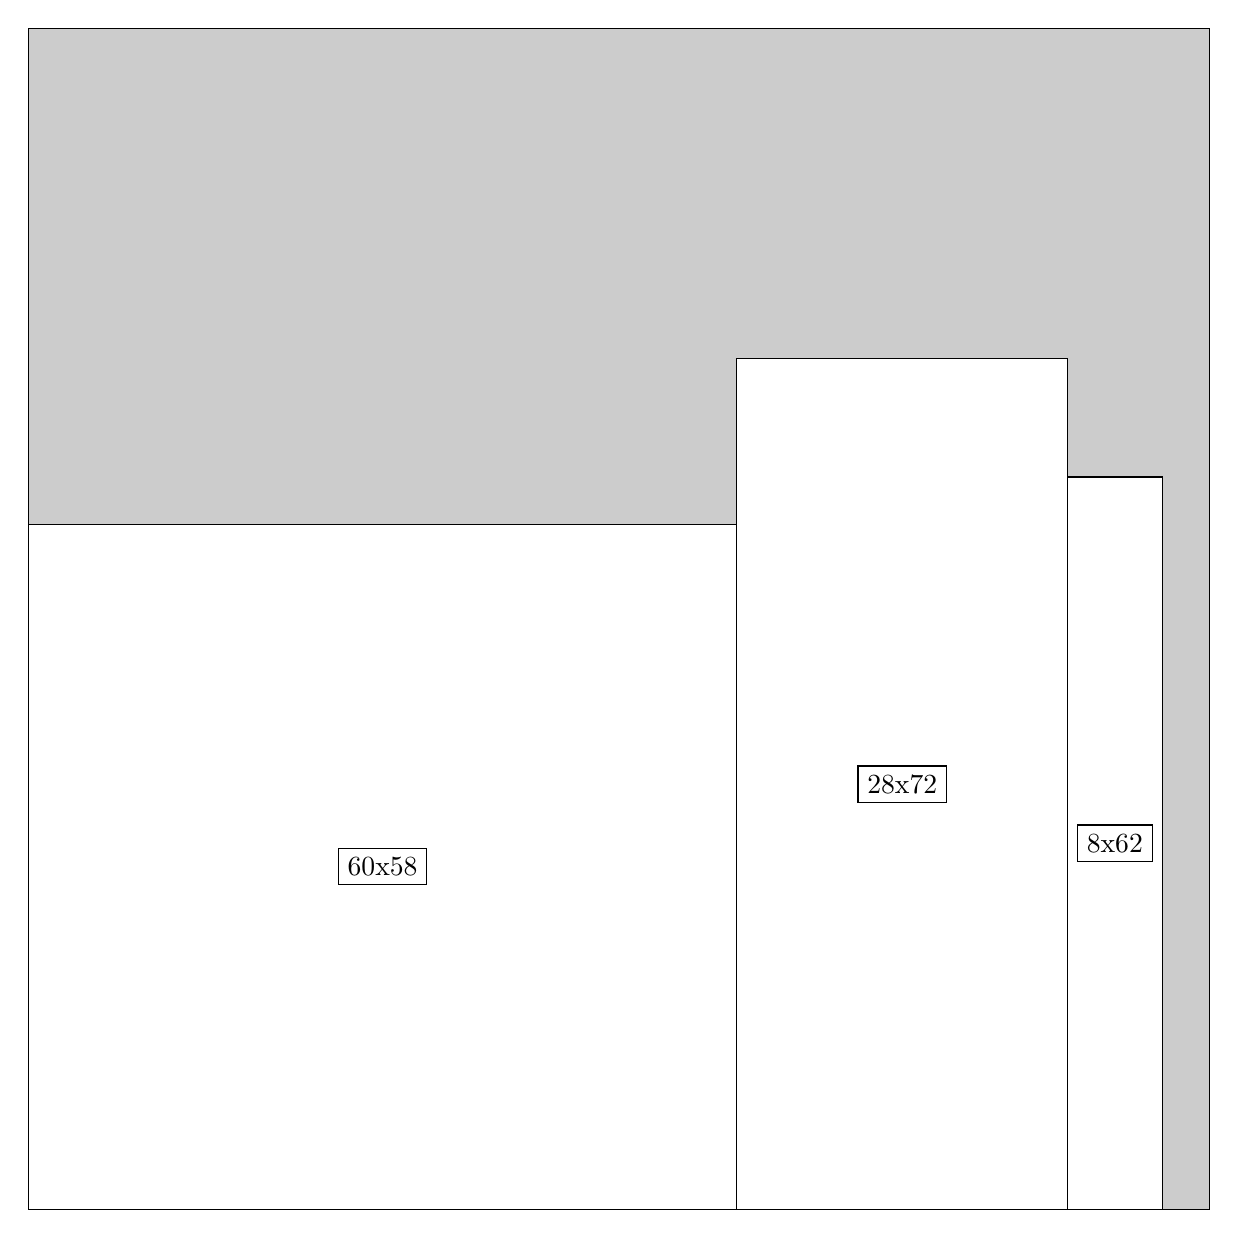
\begin{tikzpicture}[shorten >=1pt,scale=1.0,every node/.style={scale=1.0},->]
\tikzstyle{vertex}=[circle,fill=black!25,minimum size=14pt,inner sep=0pt]
\filldraw[fill=gray!40!white, draw=black] (0,0) rectangle (15.0,15.0);
\foreach \name/\x/\y/\w/\h in {28x72/9.0/0.0/4.2/10.799999999999999,60x58/0.0/0.0/9.0/8.7,8x62/13.2/0.0/1.2/9.299999999999999}
\filldraw[fill=white!40!white, draw=black] (\x,\y) rectangle node[draw] (\name) {\name} ++(\w,\h);
\end{tikzpicture}


w =28 , h =72 , x =60 , y =0 , v =2016
\par
w =60 , h =58 , x =0 , y =0 , v =3480
\par
w =8 , h =62 , x =88 , y =0 , v =496
\par
\newpage


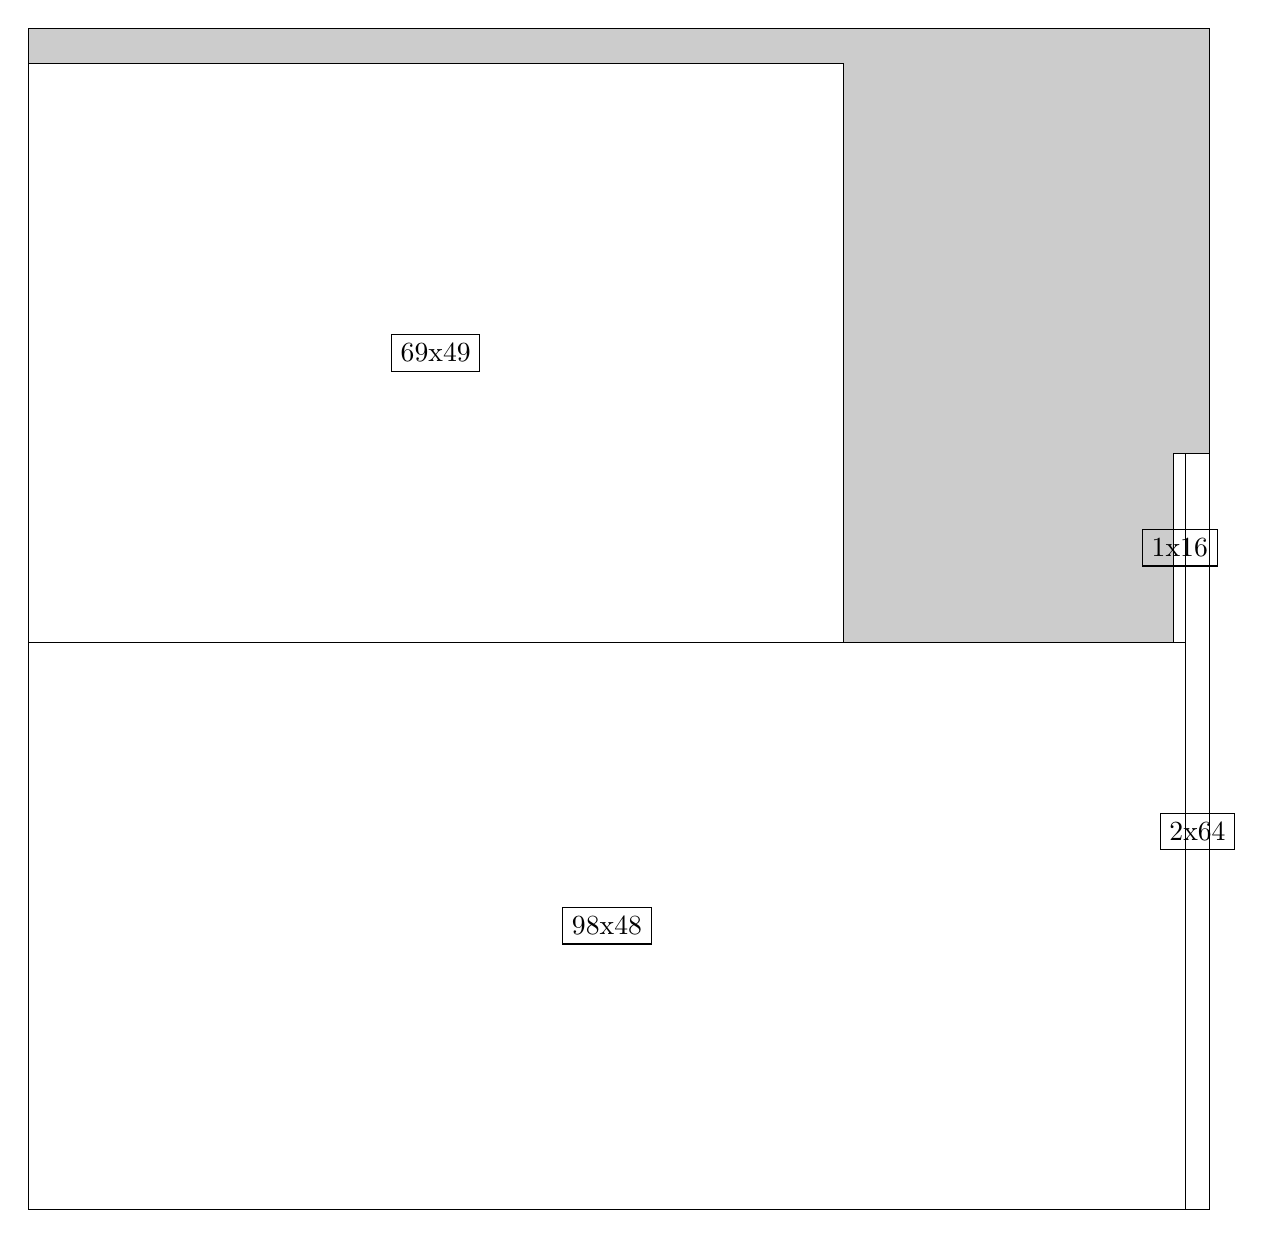
\begin{tikzpicture}[shorten >=1pt,scale=1.0,every node/.style={scale=1.0},->]
\tikzstyle{vertex}=[circle,fill=black!25,minimum size=14pt,inner sep=0pt]
\filldraw[fill=gray!40!white, draw=black] (0,0) rectangle (15.0,15.0);
\foreach \name/\x/\y/\w/\h in {98x48/0.0/0.0/14.7/7.199999999999999,69x49/0.0/7.199999999999999/10.35/7.35,2x64/14.7/0.0/0.3/9.6,1x16/14.549999999999999/7.199999999999999/0.15/2.4}
\filldraw[fill=white!40!white, draw=black] (\x,\y) rectangle node[draw] (\name) {\name} ++(\w,\h);
\end{tikzpicture}


w =98 , h =48 , x =0 , y =0 , v =4704
\par
w =69 , h =49 , x =0 , y =48 , v =3381
\par
w =2 , h =64 , x =98 , y =0 , v =128
\par
w =1 , h =16 , x =97 , y =48 , v =16
\par
\newpage


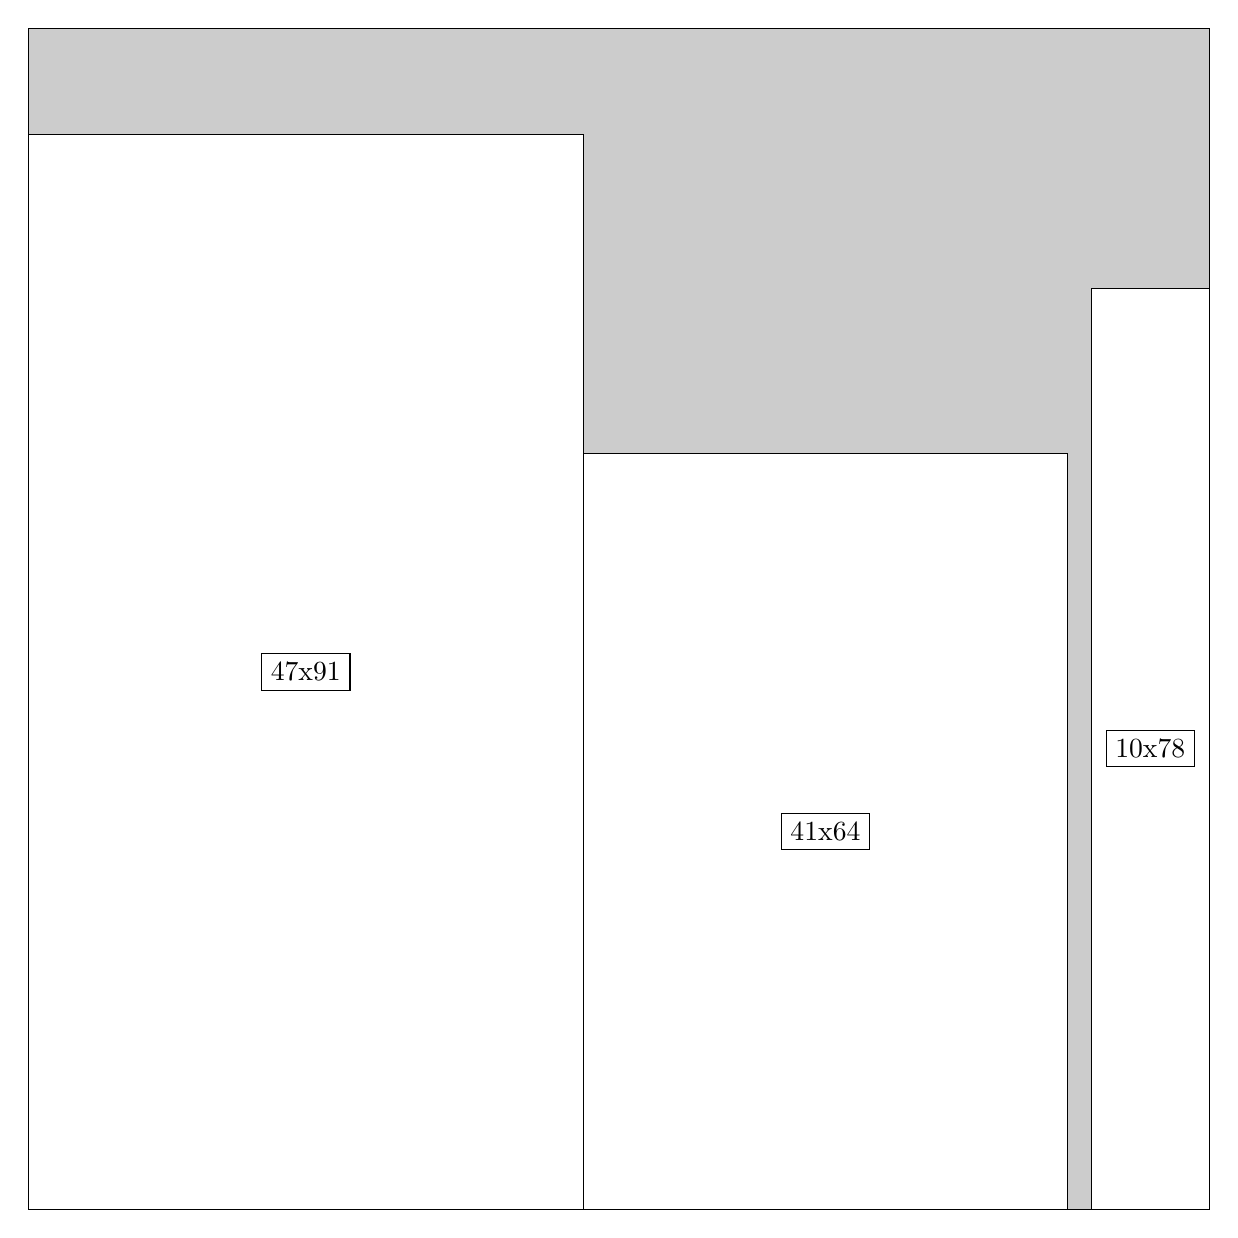
\begin{tikzpicture}[shorten >=1pt,scale=1.0,every node/.style={scale=1.0},->]
\tikzstyle{vertex}=[circle,fill=black!25,minimum size=14pt,inner sep=0pt]
\filldraw[fill=gray!40!white, draw=black] (0,0) rectangle (15.0,15.0);
\foreach \name/\x/\y/\w/\h in {47x91/0.0/0.0/7.05/13.65,41x64/7.05/0.0/6.1499999999999995/9.6,10x78/13.5/0.0/1.5/11.7}
\filldraw[fill=white!40!white, draw=black] (\x,\y) rectangle node[draw] (\name) {\name} ++(\w,\h);
\end{tikzpicture}


w =47 , h =91 , x =0 , y =0 , v =4277
\par
w =41 , h =64 , x =47 , y =0 , v =2624
\par
w =10 , h =78 , x =90 , y =0 , v =780
\par
\newpage


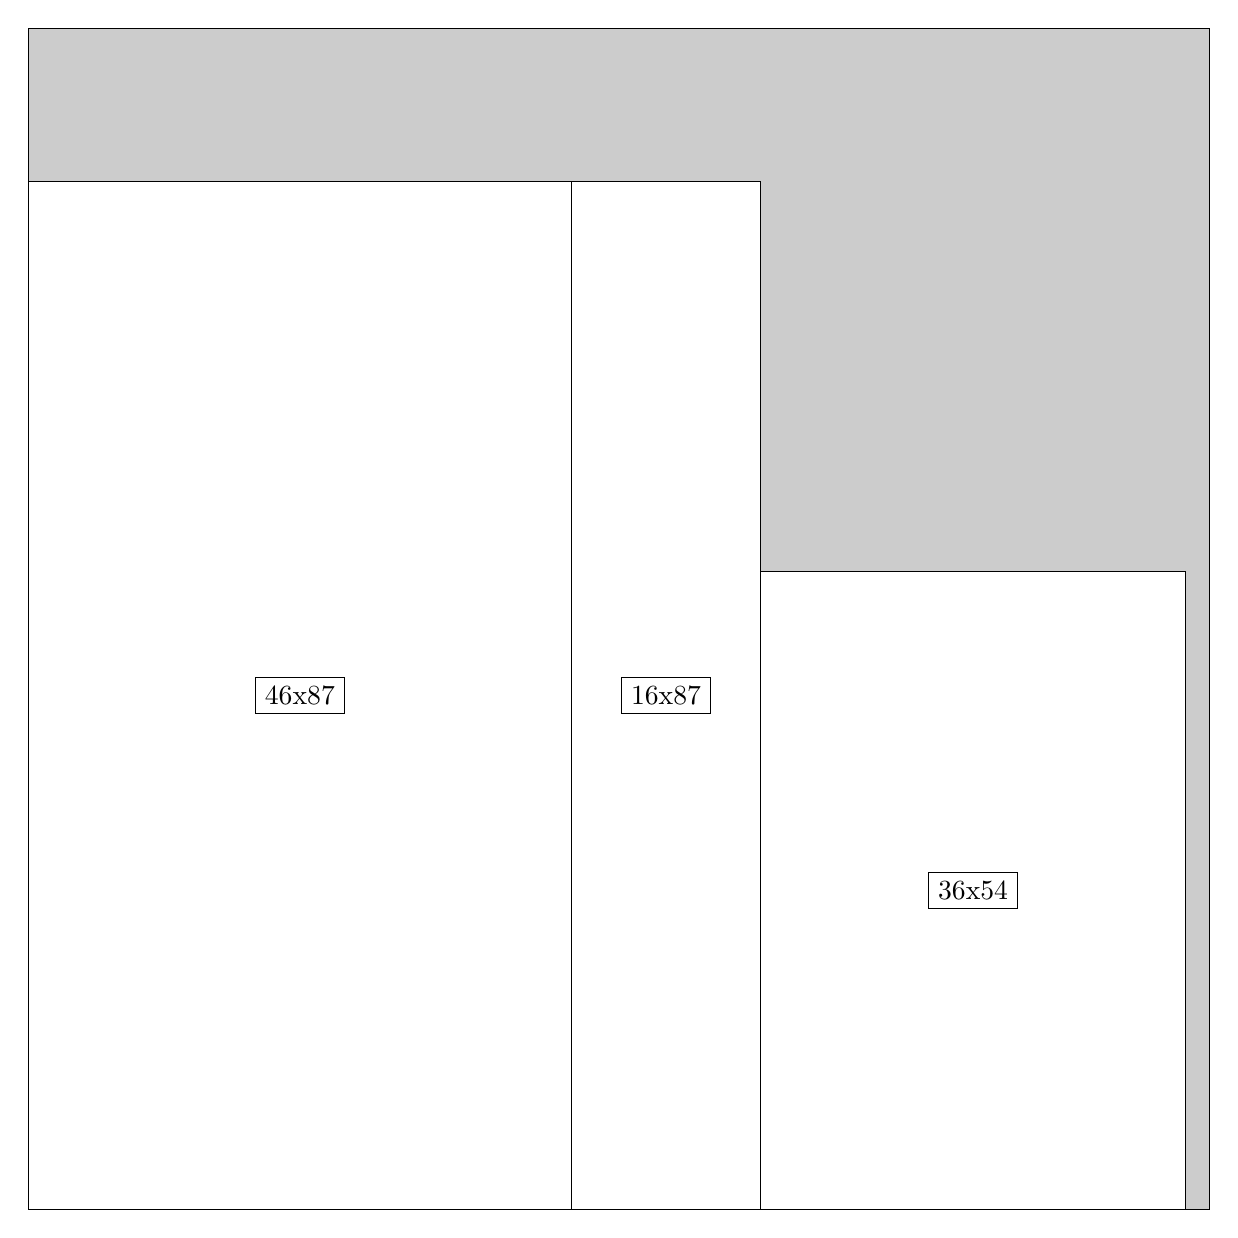
\begin{tikzpicture}[shorten >=1pt,scale=1.0,every node/.style={scale=1.0},->]
\tikzstyle{vertex}=[circle,fill=black!25,minimum size=14pt,inner sep=0pt]
\filldraw[fill=gray!40!white, draw=black] (0,0) rectangle (15.0,15.0);
\foreach \name/\x/\y/\w/\h in {46x87/0.0/0.0/6.8999999999999995/13.049999999999999,36x54/9.299999999999999/0.0/5.3999999999999995/8.1,16x87/6.8999999999999995/0.0/2.4/13.049999999999999}
\filldraw[fill=white!40!white, draw=black] (\x,\y) rectangle node[draw] (\name) {\name} ++(\w,\h);
\end{tikzpicture}


w =46 , h =87 , x =0 , y =0 , v =4002
\par
w =36 , h =54 , x =62 , y =0 , v =1944
\par
w =16 , h =87 , x =46 , y =0 , v =1392
\par
\newpage


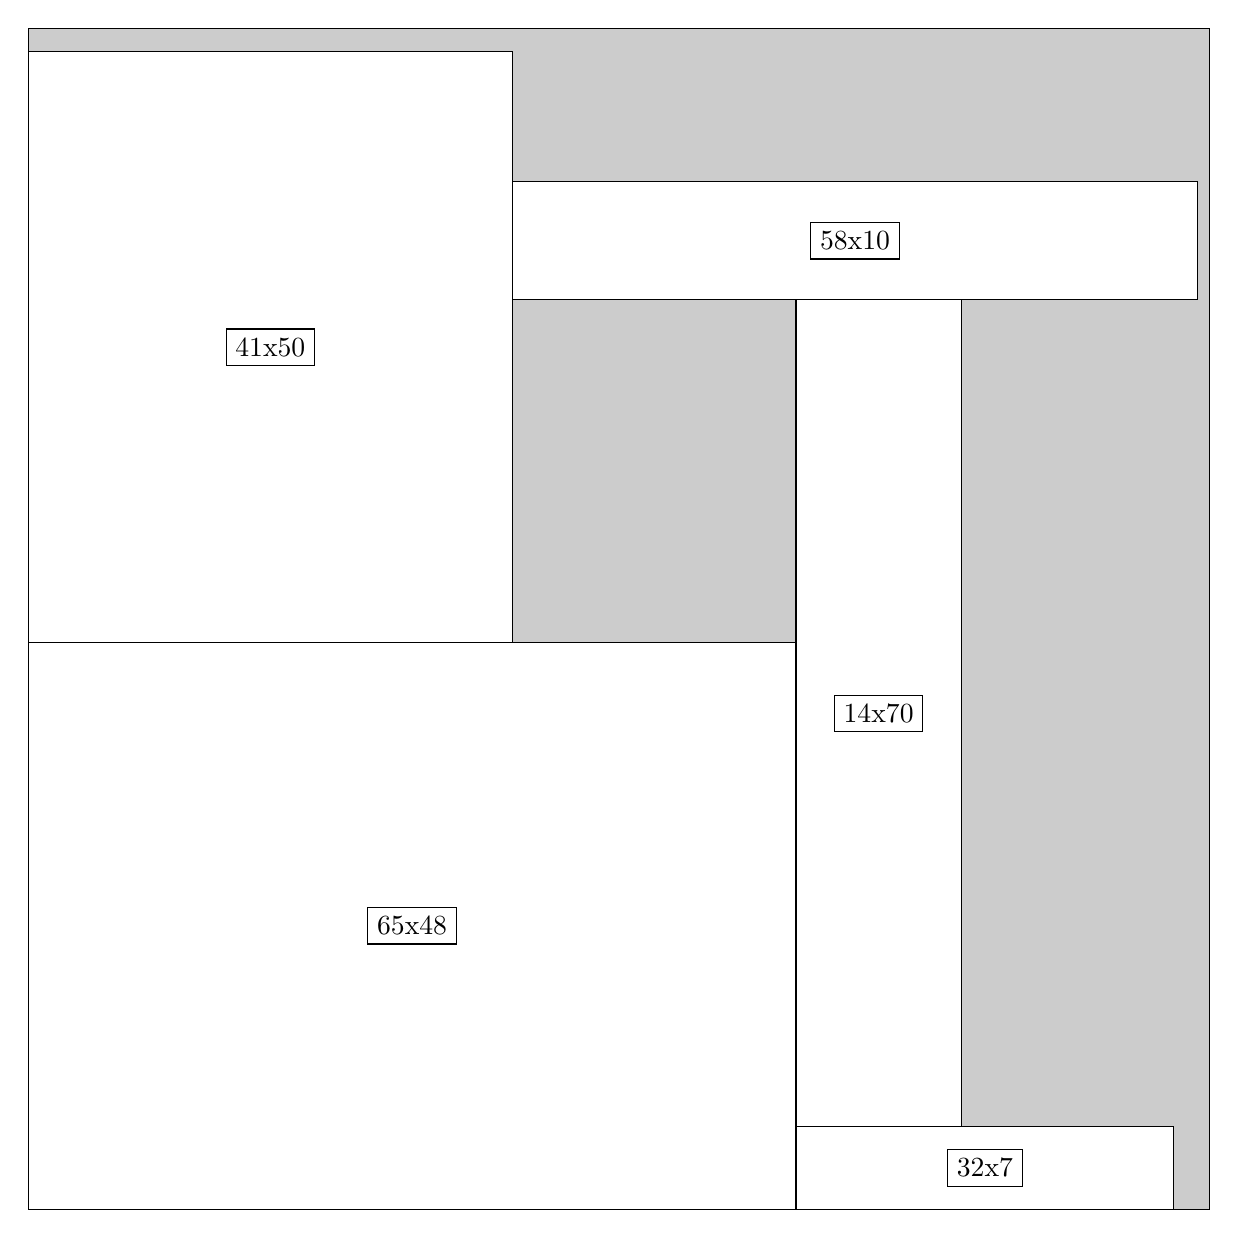
\begin{tikzpicture}[shorten >=1pt,scale=1.0,every node/.style={scale=1.0},->]
\tikzstyle{vertex}=[circle,fill=black!25,minimum size=14pt,inner sep=0pt]
\filldraw[fill=gray!40!white, draw=black] (0,0) rectangle (15.0,15.0);
\foreach \name/\x/\y/\w/\h in {65x48/0.0/0.0/9.75/7.199999999999999,41x50/0.0/7.199999999999999/6.1499999999999995/7.5,14x70/9.75/1.05/2.1/10.5,58x10/6.1499999999999995/11.549999999999999/8.7/1.5,32x7/9.75/0.0/4.8/1.05}
\filldraw[fill=white!40!white, draw=black] (\x,\y) rectangle node[draw] (\name) {\name} ++(\w,\h);
\end{tikzpicture}


w =65 , h =48 , x =0 , y =0 , v =3120
\par
w =41 , h =50 , x =0 , y =48 , v =2050
\par
w =14 , h =70 , x =65 , y =7 , v =980
\par
w =58 , h =10 , x =41 , y =77 , v =580
\par
w =32 , h =7 , x =65 , y =0 , v =224
\par
\newpage


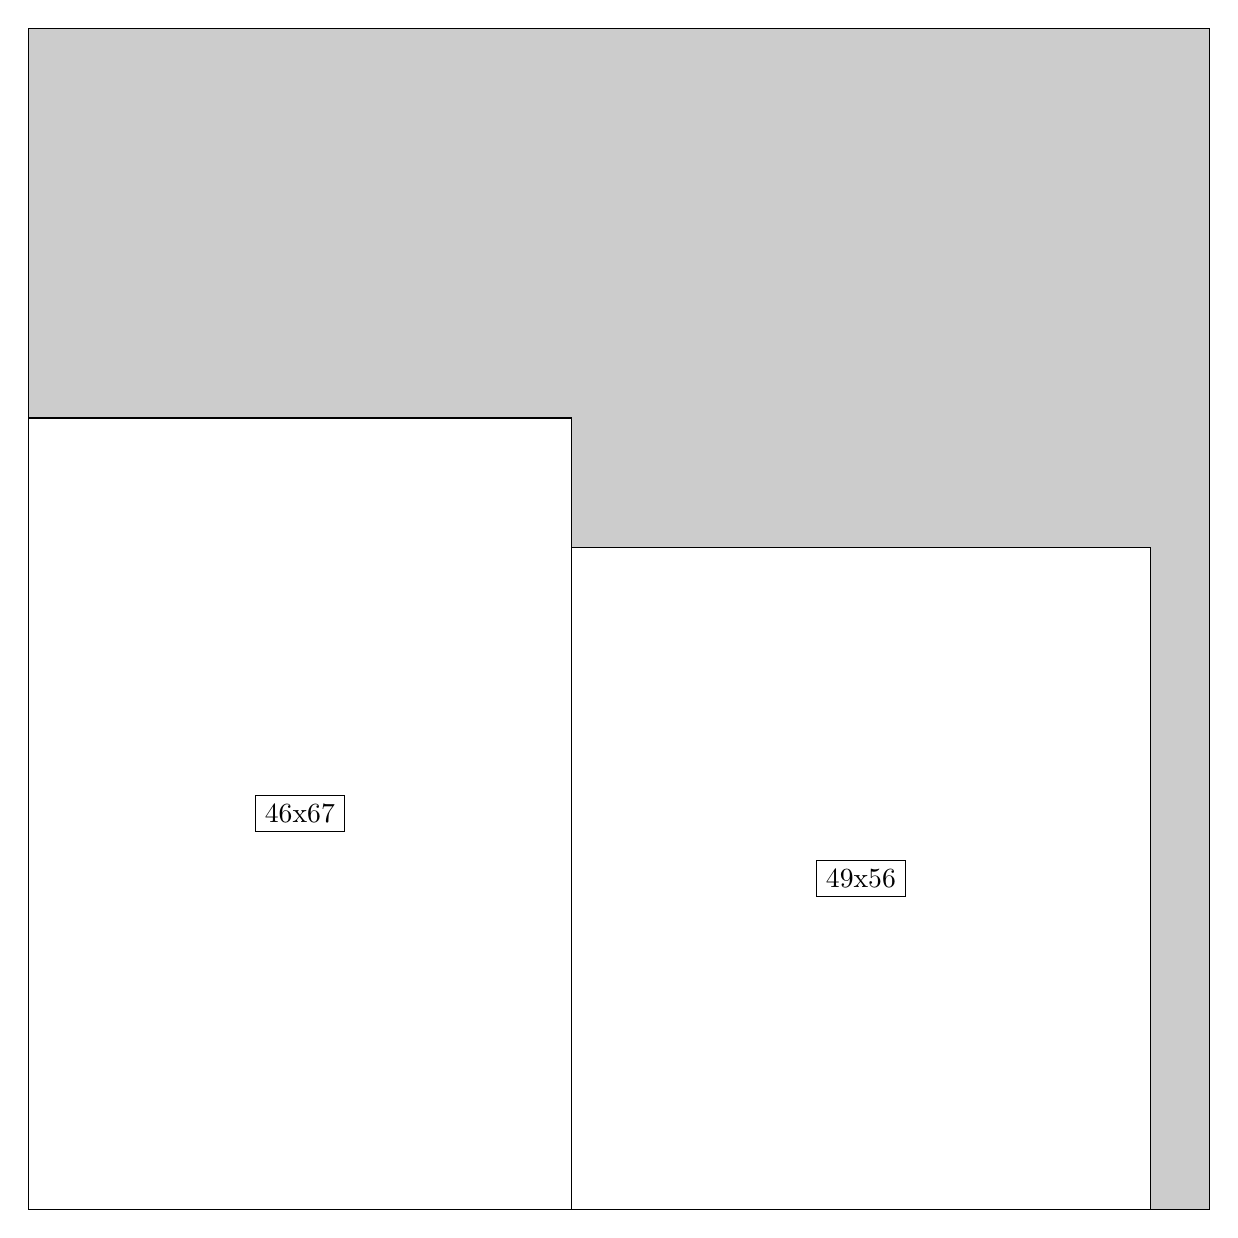
\begin{tikzpicture}[shorten >=1pt,scale=1.0,every node/.style={scale=1.0},->]
\tikzstyle{vertex}=[circle,fill=black!25,minimum size=14pt,inner sep=0pt]
\filldraw[fill=gray!40!white, draw=black] (0,0) rectangle (15.0,15.0);
\foreach \name/\x/\y/\w/\h in {46x67/0.0/0.0/6.8999999999999995/10.049999999999999,49x56/6.8999999999999995/0.0/7.35/8.4}
\filldraw[fill=white!40!white, draw=black] (\x,\y) rectangle node[draw] (\name) {\name} ++(\w,\h);
\end{tikzpicture}


w =46 , h =67 , x =0 , y =0 , v =3082
\par
w =49 , h =56 , x =46 , y =0 , v =2744
\par
\newpage


\end{document}